%\RequirePackage{lineno}

\documentclass[aps,prc,preprint,superscriptaddress,showpacs,showkeys,amsmath]{revtex4-1}
%\documentclass[article,showpacs,preprintnumbers,amsmath,amssymb]{revtex4}
\usepackage{graphicx}
\usepackage[usenames,dvipsnames,svgnames,table]{xcolor}
\usepackage{rotating}
\usepackage{graphicx}% Include  files
\usepackage{dcolumn}% Align table columns on decimal point
\usepackage{bm}% bold math
\usepackage{epsfig}
\usepackage{hyperref}
\usepackage{ulem}
\usepackage{appendix}
\begin{document}

\newcommand{\Jpsi}{J/\psi}
\newcommand{\pT}{p_{T}}
\newcommand{\calO}{{\cal{O}}}
\newcommand{\barQ}{{\bar{Q}}}
\newcommand{\barq}{{\bar{q}}}
\newcommand{\barc}{{\bar{c}}}
\newcommand{\barb}{{\bar{b}}}
\newcommand{\baru}{\bar{u}}
\newcommand{\barv}{\bar{v}}
\newcommand{\barup}{\bar{u}_{+}}
\newcommand{\barum}{\bar{u}_{-}}
\newcommand{\barvp}{\bar{v}_{+}}
\newcommand{\barvm}{\bar{v}_{-}}
\newcommand{\charm}{{\rm{charm}}}
\newcommand{\bottom}{{\rm{bottom}}}

\newcommand{\cs}{{\hat{s}}}
\newcommand{\ct}{{\hat{t}}}
\newcommand{\cu}{{\hat{u}}}
\newcommand{\alphas}{{\alpha_{s}}}

%\newcommand{}{{}}

\newcommand{\shat}{\hat{\rm s}}
\newcommand{\that}{\hat{\rm t}}
\newcommand{\uhat}{\hat{\rm u}}
\newcommand{\zhat}{\hat{\rm z}}

\newcommand{\CA}{{\cal A}}
\newcommand{\Qbar}{{\overline Q}}
\newcommand{\QQbaroctetgen}{{Q\Qbar[ ^{2S+1}L_J^{(8)}]}}
\newcommand{\QQbaroctetsingS}{{Q\Qbar[ ^1S_0^{(8)}]}}
\newcommand{\QQbaroctettripP}{{Q\Qbar[ ^3P_J^{(8)}]}}
\newcommand{\QQbaroctettripPone}{{Q\Qbar[ ^3P_1^{(8)}]}}

\def\QQbaroctettripS{Q\Qbar[ ^3S_1^{(8)}]}
\def\QQbaroctetPzero{Q\Qbar[ ^3P_0^{(8)}]}
\def\QQbaroctetPone{Q\Qbar[ ^3P_1^{(8)}]}
\def\QQbaroctetPtwo{Q\Qbar[ ^3P_2^{(8)}]}

%\newcommand{\hatt}{\hat{t}}
%\newcommand{\hatu}{\hat{u}}
%\newcommand{\hats}{\hat{s}}


%\linenumbers
\title{{\Large Charmonia production in pp collisions under NRQCD formalism}} 
\author{\large Vineet Kumar}
\author{\large Prashant Shukla}
\email{pshukla@barc.gov.in}
\affiliation{Nuclear Physics Division, Bhabha Atomic Research Center, Mumbai, India}
\affiliation{Homi Bhabha National Institute, Anushakti Nagar, Mumbai, India}
%\author{\large Ramona Vogt}
%\affiliation{Nuclear and Chemical Sciences Division, Lawrence Livermore National Laboratory, Livermore, CA 94551, USA}
%\affiliation{Physics Department, University of California, Davis, CA 95616, USA}

\date{\today}

\begin{abstract}
  In this work we calculate the high p$_{T}$ quarkonia production cross section 
  using NRQCD formalism. In NRQCD formalism quarkonia cross-section can be written 
  as a product of short distance QCD cross-sections and long distance matrix elements (LDMEs). 
  The short distance cross-sections can be calculated in terms of perturbative QCD and LDMEs are obtained 
  using experimental data.  We use measured data of $\psi$(2S), $\chi_{\rm c}$ and J/$\psi$ 
  at 1.8, 1.96, 7 and 8 TeV to  constrin LDMEs. These LDMEs are then used to calculate charmonia 
  cross-section at 13 and 14 TeV.
  %Different methods of quarkonia suppression are used to explain the high
  %p$_{T}$ quarkonia suppression obseved by CMS in LHC
\end{abstract}

\pacs{12.38.Mh, 24.85.+p, 25.75.-q}
\keywords{quark-gluon plasma, quarkonia, suppression, regeneration}

\maketitle

%%%%%%%%%%%%%%%%%%%%%%%%%%%%%%%%%%%%%%%%%%%%%%%%%%%%%%%%%%%%%%%%%%%%%%%%%%%%%%%%%%%%%%%%%%%%%%%%%%%%%%%%%%%%%%%%%

\section{Introduction}
The study of quarkonia has yielded valuable insight into the nature of the strong 
interaction ever since the discovery of the J/$\psi$ resonance~\cite{Augustin:1974xw,Aubert:1974js}. 
During the past three decades,$Q\bar Q$ bound states have provided useful laboratories 
for probing both perturbative and nonperturbative aspects of QCD. Quarkonia bound states are qualitatively 
different from most other hadrons since they are inherently nonrelativistic. 
The physics of quarkonia consequently involves several energy scales which are separated by the small velocity $v$ of the heavy 
constituents inside $Q\bar Q$ bound states.
In general one can subdivide the quarkonia production process into two major parts
\begin{enumerate}
\item Production of a heavy quark pair in hard collisions.
\item Formation of quarkonia out of the two heavy quarks.
\end{enumerate}
Due to the high mass of the heavy quarks (m$_{\rm c}\,\sim$ 1.5 GeV/c$^2$, m$_{\rm b}\,\sim$ 4.5 GeV/c$^2$), 
they can be produced only during the first phase of a collision.
Only at that time the elementary collisions with sufficiently high momentum 
transfers (to create such high masses) takes place. For this reason the heavy quark production
is a hard process that can be treated perturbatively~\cite{Nason:1987xz,Nason:1989zy}, while the formation
of quarkonia out of the two heavy quarks is a non purterbative process.
%and require some effective theories for modeling.
The nonperturbative evolution of the $Q\bar Q$ pair into a quarkonium
has been discussed extensively in terms of models and in terms of the
language of effective theories of QCD
\cite{Bodwin:1994jh,Brambilla:2004wf}. Different
treatments of this evolution have led to various theoretical models for
inclusive quarkonium production. Most notable among these are the color-singlet
model (CSM), the color-evaporation model (CEM), the non-relativistic QCD
(NRQCD) factorization approach, and the fragmentation-function approach.

The CSM was first proposed shortly after the discovery of the J/$\psi$
\cite{Einhorn:1975ua,Ellis:1976fj,Carlson:1976cd,Berger:1980ni}.
In this model, it is assumed that the $Q\bar Q$ pair that evolves into
the quarkonium is in a color-singlet state and that it has the same spin
and angular-momentum quantum numbers as the quarkonium. In the CSM, the
production rate for each quarkonium state is related to the absolute
values of the color-singlet $Q\bar Q$ wave function and its derivatives,
evaluated at zero $Q\bar Q$ separation. These quantities can be
extracted by comparing theoretical expressions for quarkonium decay
rates in the CSM with experimental measurements. Once this extraction
has been carried out, the CSM has no free parameters. The CSM was
successful in predicting quarkonium production rates at relatively low
energy \cite{Schuler:1994hy}. Recently, it has been found that, at high
energies, very large corrections to the CSM appear at next-to-leading
order (NLO) and next-to-next-to-leading order (NNLO) in $\alpha_s$
\cite{Artoisenet:2007xi,Campbell:2007ws,Artoisenet:2008fc}.
Consequently, the possibility that the CSM might embody an important 
production mechanism at high energies has re-emerged. 
However, given the very large corrections at
NLO and NNLO, it is not clear that the perturbative expansion in
$\alpha_s$ is convergent. 
%Furthermore, in the production and decay of
%$P$-wave and higher-orbital-angular-momentum quarkonium states, the CSM
%is known to be inconsistent because it leads to uncanceled infrared
%divergences. (See Ref.~\cite{Brambilla:2004wf} and references therein.)
As we will describe below, the NRQCD factorization approach encompasses
the color-singlet model, but goes beyond it.

The CEM~\cite{Fritzsch:1977ay,Amundson:1995em,Amundson:1996qr}
is motivated by the principle of quark-hadron duality. In the CEM, it
is assumed that every produced $Q\bar Q$ pair evolves into a quarkonium
if it has an invariant mass that is less than the threshold for
producing a pair of open-flavor heavy mesons. It is further assumed that
the nonperturbative probability for the $Q\bar Q$ pair to evolve into a
quarkonium state $H$ is given by a constant $F_H$ that is
energy-momentum and process independent. Once $F_H$ has been fixed by
comparison with the measured total cross section for the production of
the quarkonium $H$, the CEM can predict, with no additional free
parameters, the momentum distribution of the quarkonium production rate. The
CEM predictions provide good descriptions of the CDF data for J/$\psi$,
$\psi$(2S), and $\chi_{\rm c}$ production at $\sqrt{s}=1.8$~TeV
\cite{Amundson:1996qr}. The CEM model has a full predicting power about 
cross-sections but it fails to predict the quarkonium polarization.

In the fragmentation-function approach the inclusive
quarkonium production cross sections is written  
in terms of convolutions of parton production cross sections 
with light-cone fragmentation functions~\cite{Nayak:2005rw,Nayak:2005rt}.
This procedure provides a convenient way to organize the contributions
to the cross section in terms of powers of $m_Q/p$.
The contribution to the cross section at the
leading power in $m_Q/p_T$ is given by the production of a single parton
({\it e.g.}, a gluon), at a distance scale of order $1/p_T$, which
subsequently fragments into a heavy quarkonium
\cite{Braaten:1996pv}.  The contribution to the cross section at the
first sub-leading power in $m_Q/p_T$ is given by the production of a
$Q\bar Q$ pair in a vector- or axial-vector state, at a distance scale of
order $1/p_T$, which then fragments into a heavy quarkonium.

The NRQCD factorization approach \cite{Bodwin:1994jh} to
heavy-quarkonium production is by far the most sound theoretically
and most successful phenomenologically. 
%The NRQCD factorization approach 
%implies a separation of process-dependent 
%short-distance coefficients, to be calculated perturbatively as
%expansions in the strong-coupling constant $\alpha_s$, from supposedly 
%universal LDMEs, to be extracted from experiment.
The NRQCD factorization approach 
expresses the probability for a $Q\bar Q$ pair to evolve into a quarkonium 
in terms of matrix elements of NRQCD operators. These matrix elements can be 
characterized in terms of their scaling with the heavy-quark velocity $v$ in the limit $v\,\ll\,1$.
A crucial feature of this formalism is that it takes into account the complete structure of the 
$Q\bar Q$ Fock space, which is spanned by the state $n\,=\,^{2S+1}L_{J}^{[a]}$ with definite spin $S$, 
orbital angular momentum $L$, total angular momentum $J$, and color multiplicity a = 1, 8. In particular, 
this formalism predicts the existence of Color Octet (CO) processes in nature. This means that 
$Q\bar Q$ pairs are produced at short distances in CO states and subsequently evolve into 
physical, color-singlet (CS) quarkonia by the nonperturbative emission of soft gluons. 
In the limit $v\rightarrow0$, the traditional CS model (CSM) is recovered in the 
case of S-wave quarkonia

%%%NLO Stuff
In last few years, there is some very important progress in the NLO QCD correction 
calculation. The NLO corrections to color-singlet (CS) J/$\psi$ hadroproduction 
have been investigated in Ref.~\cite{Campbell:2007ws,Gong:2008sn}. its transverse momentum distribution is 
found to be enhanced by 2-3 order of magnitude at high p$_t$ region, and its 
polarization changes from transverse into longitudinal at NLO~\cite{Gong:2008sn}.The
NLO corrections to J/$\psi$ production via S-wave color octet (CO) states 
($^1S_{0}^{[8]}\,^3S_{1}^{[8]}$) are studied in Ref.~\cite{Gong:2008ft} and the corrections 
to p$_{t}$ distributions of both J/$\psi$ yield and polarization are found to be small. 
In Refs.~\cite{Ma:2010vd}, NLO corrections for $\chi_{cJ}$ hadroproduction are studied.
%The calculation for polarization of direct J/$\psi$ hadroproduction at NLO QCD 
%was presented by two groups~\cite{Butenschoen:2012px,Chao:2012iv}

The test of NRQCD factorization has been identified among the most critical
milestones on the roadmap of quarkonium physics at the present time. While, for
J/$\psi$ polarization, comparisons of measured data with NRQCD predictions,
unravel a rather confusing pattern~\cite{Butenschoen:2012px,Chao:2012iv,Gong:2012ug}, the situation is 
better for the J/$\psi$ yield~\cite{Gong:2012ug,Butenschoen:2010rq,Ma:2010jj}. It has been shown 
that the set of CO LDMEs fitted to transverse-momentum (p$_{T}$ ) distributions
measured at HERA and CDF lead to very good descriptions of 
the p$_{T}$ distributions from RHIC and the LHC~\cite{Butenschoen:2010rq} 
On the other hand, the Tevatron data alone is not sufficient to constrain
all the CO LDMEs~\cite{Ma:2010jj} also the fit results of 
Ref.~\cite{Butenschoen:2010rq} and  Ref~\cite{Ma:2010jj} are incompatible with 
eachother.

After the continuous running of LHC for several years we now enter the era 
of precise quarkonia measurements. We now have very high quality quarkonia 
production data in several kinamatic 
regions up to very high transeverse momentum. In this paper we use this new
data from LHC~\cite{Chatrchyan:2011kc,Khachatryan:2015rra,Aad:2015duc} along with 
the available data from CDF~\cite{Acosta:2004yw,Abe:1997yz} to constrain 
the LDMEs. These new LDMEs are then used to predict the J/$\psi$ and $\psi$(2S)
cross-section at 13 TeV for the kinematical bins relevant to LHC detectors.



%Heavy-ion collisions at relativistic energies are performed to create and characterize 
%quark gluon plasma (QGP), a phase of strongly-interacting matter at high energy density 
%where quarks and gluons are no longer bound within hadrons.
%The quarkonia states ($\Jpsi$ and $\Upsilon$) have been some of the most popular tools 
%since their suppression was proposed as a signal of QGP formation \cite{Matsui:1986dk}.
%The understanding of these probes has evolved substantially via measurements 
%through three generations of experiments: the SPS (at CERN), RHIC (at BNL) and the LHC (at CERN) 
%and by a great deal of theoretical activity. (For recent reviews see 
%Refs.~\cite{Schukraft:2013wba,Kluberg:2009wc,Brambilla:2010cs}.)
%Quarkonia are produced early in the heavy-ion collisions and, if they evolve
%through the deconfined medium, their yields should be suppressed in comparison with those in $pp$ collisions. \\
%{\color{red} To be written .....}

%%%%%%%%%%%%%%%%%%%%%%%%%%%%%%%%%%%%%%%%%%%%%%%%%%%%%%%%%%%%%%%%%%%%%%%%%%%%%%%%%%%%%%%
\section{Quarkonia Production in p$+$p collisions}
\label{section:ppProduction}
The factorization formalism of the NRQCD  provides a theoretical framework for 
studying the heavy quarkonium production. The dominant processes in evaluating 
the differential yields of heavy mesons $\psi$ as a function of $p_T$ are the $2\rightarrow 2$
processes of the kind $g+q\rightarrow \psi+q$, $q+\bar{q}\rightarrow \psi+g$ and
$g+g\rightarrow \psi+g$, where $\psi$ refers to the heavy meson. We label the process
generically as $a+b\rightarrow \psi+X$, where $a$ and $b$ are the light incident
partons. The invariant cross-section can be written in factorized form as 
\begin{equation}
  %\begin{split}
    E\frac{d^{3}\sigma^{\psi}}{d^{3}p} = \sum_{a,b}\int \int dx_a\,dx_b 
    G_{a/p}(x_a,\mu_{F}^{2}) G_{b/p}(x_b,\mu_{F}^{2})\frac{\hat s}{\pi}\frac{d\sigma}{d\hat t}
    \otimes \delta(\hat s + \hat t + \hat u -M^{2}) 
%\end{split}
\label{eqn:cross}
\end{equation}
where, $G_{a/p}(G_{b/p})$ is the parton distribution function (PDF) of the incoming parton $a(b)$ in the 
incident proton, which depends on the momentum fraction $x_a(x_b)$ and the factorization 
scale $\mu_F$ as well as on the renormalization scale $\mu_R$. However, 
as we have chosen $\mu_F$ = $\mu_R$, in our case PDFs are function of $x$ and $\mu_F$ only. 
The parton level cross-section d$\sigma$/d$\hat{t}$ is defined as~\cite{}
\begin{equation}
\frac{d\sigma}{d\hat t} = \frac{d\sigma}{d\hat t}(ab\rightarrow Q\overline{Q}(^{2S+1}L_{J})+X)\,M_{L}(Q\overline{Q}(^{2S+1}L_{J})\rightarrow\psi)
\end{equation}
The short distance contribution $d\sigma/d\hat t (ab\rightarrow Q\overline{Q}(^{2S+1}L_{J})+X)$ can be calculated within 
the framework of perturbative QCD (pQCD). $M_{L}(Q\overline{Q}(^{2S+1}L_{J})\rightarrow\psi)$ are the nonperturbative 
LDMEs and can only be estimated by comparison with experimental measurements. 
For $a+b\rightarrow \psi+X$ kind of processes the parton level  Mandelstam variables ${\hat s}$, ${\hat t}$, and ${\hat u}$
can be expressed in terms of $x_a$, $x_b$ as 
%At this stage, the integration upon $x_b$ can be performed using the properties of delta function. 
%To solve the integration we have to express the ${\hat s}$, ${\hat t}$, and ${\hat u}$
%in terms of $x_a$, $x_b$, resonance transeverse momentum $p_{T}$ and rapidity $y$. 
%For $ab\rightarrow \psi+X$ kind of processes following are the relations between ${\hat s}$, ${\hat t}$, ${\hat u}$ 
%and meson variables  
\begin{equation}
\begin{split}
\cs = \,&x_{a}\,x_{b}\,s \\
\ct = \,&M^{2} - x_{a}\,\sqrt{s}\,m_{T}\,e^{-y}\\
\cu = \,&M^{2} - x_{b}\,\sqrt{s}\,m_{T}\,e^{y}\\
 \end{split}  
\end{equation}
where, $\sqrt{s}$ being the total energy in the centre-of-mass and $y$ is the rapidity and $p_{T}$ is the
transverse momentum of the $Q\bar Q$. Writing down $ \hat s + \hat t + \hat u -M^{2} = 0$ and solving for $x_{b}$ we obtain
\begin{equation}
x_b = \frac{1}{\sqrt{s}}\frac{x_a\,\sqrt{s}\,m_T\,e^{-y}-m^2_H}{x_a\,\sqrt{s}-m_T\,e^y}.
\end{equation}
The double differential cross-section upon $p_{T}$ and y takes the following form
\begin{equation}
  \frac{{d^{2}\sigma}^{ab\rightarrow cd}}{dp_T\,dy} = \sum_{a,b}\int_{x_{a}^{min}}^{1} dx_a\, G_{a/A}(x_a,\,\mu^{2}_{F})\, G_{b/B}(x_b,\,\mu^{2}_{F})\times 
  2p_T \frac{x_a\,x_b}{x_a-\frac{m_T}{\sqrt{s}}e^y}\frac{d\sigma}{d\hat t},
\end{equation}
The minimum value of $x_a$ is 
\begin{equation}
x_{a\rm min} = \frac{1}{\sqrt{s}}\frac{\sqrt{s}\,m_T\,e^{y}-m^2_H}{\sqrt{s}-m_T\,e^{-y}}.
\end{equation}
The short distance invariant differential cross-section is given by
\begin{equation}
  \frac{d\sigma}{d\hat t}(ab\rightarrow Q\overline{Q}(^{2S+1}L_{J})+X) = \frac{|\mathcal{M}|^2}{16\pi{\hat s}^2},
\end{equation}
$|\mathcal{M}|^2$ is the feynman squared amplitude averaged over initial spin of partons.  In our calculations, we use the expressions 
for the short distance Color Singlet (CS) cross-sections given in Refs.~\cite{Baier:1983va,Humpert:1986cy,Gastmans:1987be} 
and the Color Octet (CO) cross-sections given in Refs.~\cite{Cho:1995vh,Cho:1995ce,Braaten:2000cm}. In our numerical computation, 
we use CTEQ6M~\cite{Lai:2010vv} for the parton distribution functions. 
The LDMEs are predicted to scale with a definite power of the relative velocity $v$ of the heavy constituents inside $Q\bar Q$ bound states. 
In the limit $v<<1$, the production of quarkonium is based on the $^3S_1^{[1]}$ and $^3P_J^{[1]}$ ($J$ = 0,1,2) CS states 
and $^1S_0^{[8]}$, $^3S_1^{[8]}$ and $^3P_J^{[8]}$ CO states.
The differential cross section for the direct production of $J/\psi$ can be written 
as the sum of the contributions,
\begin{equation}
\begin{split}
d\sigma(J/\psi) &= d\sigma(Q\barQ([^3S_1]_{1}))
                   \,M_{L}(Q\barQ([^3S_1]_{1})\rightarrow J/\psi) 
                +  d\sigma(Q\barQ([^1S_0]_{8}))
                   \,M_{L}(Q\barQ([^1S_0]_{8})\rightarrow J/\psi)\\ 
                &+  d\sigma(Q\barQ([^3S_1]_{8}))
                   \,M_{L}(Q\barQ([^3S_1]_{8})\rightarrow J/\psi) 
                +  d\sigma(Q\barQ([^3P_0]_{8}))
                   \,M_{L}(Q\barQ([^3P_0]_{8})\rightarrow J/\psi)\\ 
                &+  d\sigma(Q\barQ([^3P_1]_{8}))
                   \,M_{L}(Q\barQ([^3P_1]_{8})\rightarrow J/\psi)
                +  d\sigma(Q\barQ([^3P_2]_{8}))
                   \,M_{L}(Q\barQ([^3P_2]_{8})\rightarrow J/\psi)\\
                &+ \cdot\cdot\cdot  \;,
\label{eq:dsigmaJ}
\end{split}
\end{equation}
where the quantity in the brackets $[\;]$ represents the angular momentum
quantum numbers of the $Q\barQ$ pair in the Fock expansion. The subscript on
$[\;]$ refers to the color structure of the $Q\barQ$ pair, $1$ being 
the color-singlet and $8$ being the color-octet. The dots represent terms which contribute at
higher powers of $v$. The short distance cross sections $d\sigma(Q\barQ)$
correspond to the production of a $Q\barQ$ pair in a particular color and spin
configuration, while the long distance matrix element
$M_{L}(Q\barQ)\rightarrow J/\psi$ corresponds to the probability
of the $Q\barQ$ state to convert to the quarkonium wavefunction. This
probability includes any necessary prompt emission of soft gluons to prepare a
color neutral system that matches onto the corresponding Fock component of the
quarkonium wavefunction. 
Power counting rules tell us that contributions from the color-octet matrix
elements in Eq.~\ref{eq:dsigmaJ} are suppressed by $v^4$ compared to the color
singlet matrix elements.

The case of the $p$-wave bound states ($\chi_{c0}$, $\chi_{c1}$, and
$\chi_{c2}$, collectively referred to as $\chi_{cJ}$ is slightly different. 
The color-singlet state $Q\barQ[^3P_J]_{1}$ and the color-octet state
$Q\barQ[^3S_1]_{8}$ contribute to the same order in $v$ ($v^{5}$) because of the angular
momentum barrier for $p-$wave states, and hence both need to be included for a consistent
calculation in $v$.  For the calculation of the production cross section, we
consistently take the contributions to the lowest order in $v$.
The $\chi_{c}$ differential cross section can be written as 
\begin{equation}
\begin{split}
d\sigma(\chi_{cJ}) =\,&d\sigma(Q\barQ([^3P_J]_{1}))
                   \,M_{L}(Q\barQ([^3P_J]_{1})\rightarrow \chi_{cJ}) 
                +  d\sigma(Q\barQ([^3S_1]_{8}))
                   \,M_{L}(Q\barQ([^3S_1]_{8})\rightarrow \chi_{cJ})\\
                &+ \cdot\cdot\cdot  
\label{eq:dsigmachi}
\end{split}
\end{equation}
Similar expressions hold for the $\chi_b(1P), \chi_b(2P)$ and $\chi_b(3P)$ 
mesons. 
Using above mentioned formalism we calculate the cross-section of charmonia states 
at LHC energies. For $J/\psi$ production in $p-p$ collisions at LHC energies, three sources 
need to be considered: direct $J/\psi$ production from initial parton-parton hard scattering, 
feed-down contributions to the $J/\psi$ from the decay of heavier charmonium states, 
predominantly from $\psi(2S)$, $\chi_{c0}$, $\chi_{c1}$ and $\chi_{c2}$ and $J/\psi$ 
from $B$ hadron decays. The sum of the first two sources is called "prompt $J/\psi$" and the third source 
is called "$J/\psi$ from $B$". On the other hand, $\psi(2S)$ has no significant feed-down contributions 
from higher mass states. We call this direct contribution as "prompt $\psi(2S)$" to be consistent with 
the experiments. 
For the production of prompt $J/\psi$ we consider the direct contribution, and
feed-down contributions from $\chi_{c0}(1P)$, $\chi_{c1}(1P)$,
$\chi_{c2}(1P)$ and $\psi(2S)$. The relevant branching fractions are given
in Table~\ref{table:CharmoniaBFs},


In this work, following~\cite{Cho:1995ce,Cho:1995vh} we use the values of the
color-singlet matrix elements calculated using the potential model. The expressions
and the values for the color-singlet operators can be found in~\cite{Cho:1995ce,Cho:1995vh,Eichten:1994gt}. 
The values are obtained by solving the non-relativistic wavefunctions:
\begin{equation}
\begin{split}
 &M_{L}(c\barc([^3S_1]_{1})\rightarrow J/\psi) = 3 \,M_{L}(c\barc([^1S_0]_{1})\rightarrow J/\psi) = 3N_c\frac{|R_{n=1}(0)|^2}{2\pi} = 1.2\;{\rm GeV^3} \;, \\
 &M_{L}(c\barc([^3S_1]_{1})\rightarrow \psi(2S))=3 \,M_{L}(c\barc([^1S_0]_{1})\rightarrow \psi(2S)) =3N_c\frac{|R_{n=2}(0)|^2}{2\pi}=0.76\;{\rm GeV^3} \;, \\
 &\frac{1}{5} M_{L}(c\barc([^3P_2]_{1})\rightarrow \chi_{c2}(1P))=\frac{1}{3} \,M_{L}(c\barc([^3P_1]_{1})\rightarrow \chi_{c1}(1P)) =\,M_{L}(c\barc([^3P_0]_{1})\rightarrow \chi_{c0}(1P))\\
 &=3N_c\frac{|R^\prime_{n=1}(0)|^2}{2\pi} =0.054 \, m_{\charm}^2\;{\rm GeV^3}. 
\label{eq:charmsinglet}
\end{split}
\end{equation}
Here $R(0)$ is the radial wavefunction at the origin, $R^\prime(0)$ is the
first derivative of the radial wavefunction at the origin, and $n$ refers to
the radial quantum number. We take the mass of the charm quark, $m_{charm}=1.6$ GeV. 
The color-octet operators can not be related to the non-relativistic
wavefunctions of $Q\barQ$ since it involves a higher Fock state.
We use measured data from LHC~\cite{Chatrchyan:2011kc,Khachatryan:2015rra,Aad:2015duc} 
and TeVatron~\cite{Acosta:2004yw} to constrain these  Color Octet Matrix elements.
For the net production of $J/\psi$ we consider the direct contribution and
feed-down contributions from $\chi_{c0}(1P)$, $\chi_{c1}(1P)$,
$\chi_{c2}(1P)$ and $\psi(2S)$. 
Yields of $\psi(2S)$ have been measured at TeVatron~\cite{Abe:1997yz} and LHC~\cite{Chatrchyan:2011kc}. 
Data for $\chi_{cJ}$ is available from TeVatron~\cite{Abe:1997yz}.  

\begin{table*}[h]
\caption{Relevant branching fractions for charmonia~\cite{Nakamura:2010zzi}}
\begin{tabular}{c|cccc}
Meson From &to $\chi_{c0}$ &to $\chi_{c1}$ &to $\chi_{c2}$ &to $J/\psi$\\ 
\hline
$\psi(2S)$ & 0.0962 & 0.092 & 0.0874 & 0.595   \\
$\chi_{c0}$& &  &  & 0.0116           \\
$\chi_{c1}$& &  &  & 0.344           \\
$\chi_{c2}$& &  &  & 0.195           \\
\end{tabular}
\label{table:CharmoniaBFs}
\end{table*}

 The following color-singlet and color-octet contributions are relevant for our
calculation.


\begin{enumerate}
\item{Direct contributions
\begin{equation}
\begin{split}
&M_{L}(c\barc([^3S_1]_{1})\rightarrow J/\psi) = 1.2\,{\rm GeV}^{3}\\
&M_{L}(c\barc([^3S_1]_{8})\rightarrow J/\psi) \\
&M_{L}(c\barc([^1S_0]_{8})\rightarrow J/\psi) \\
&M_{L}(c\barc([^3P_0]_{8})\rightarrow J/\psi) \\
~\label{eq:Mpsi1}
\end{split}
\end{equation}
    }
\item{Feed-down contribution from $\psi(2S)$
\begin{equation}
\begin{split}
&M_{L}(c\barc([^3S_1]_{1})\rightarrow \psi(2S)) = 0.76\,{\rm GeV}^{3}\\
&M_{L}(c\barc([^3S_1]_{8})\rightarrow \psi(2S)) \\
&M_{L}(c\barc([^1S_0]_{8})\rightarrow \psi(2S)) \\
&M_{L}(c\barc([^3P_0]_{8})\rightarrow \psi(2S)) \\
~\label{eq:Mpsi2}
\end{split}
\end{equation}
    }
\item{Feed-down contribution from $\chi_{cJ}$
\begin{equation}
\begin{split}
&M_{L}(c\barc([^3P_0]_{1})\rightarrow \chi_{c0}) = 0.054\,m_{c}^{2}\,{\rm GeV}^{3}\\ 
&M_{L}(c\barc([^3S_1]_{8})\rightarrow \chi_{c0})\\
~\label{eq:Mchi}
\end{split}
\end{equation}
    }
\end{enumerate}
Hence for $J/\psi$ we have to determine $10$ parameters. Three color singlet matrix elements
can be estimated from the wavefunctions of the heavy mesons. 
We use the following procedure to determine the remaining
$7$ color-octet components. 
CDF~\cite{Abe:1997yz} has measured the feed-down contribution from the
$\chi_{cJ}$ states to $J/\psi$ production. We use this data to fit the color octet
matrix element $M_{L}(Q\barQ([^3S_1]_{8})\rightarrow \chi_{c0})$. Figure~\ref{Fig:LDMEChicCDF} shows
different components of cross-section along with the CDF data 
\begin{equation}
\begin{split}
M_{L}(Q\barQ([^3S_1]_{8})\rightarrow \chi_{c0})/m_{\charm}^2 &= (0.00157\pm {\color{red} 0.00159})\,{\rm GeV^3}\;,
~\label{eq:Mchicn1CO_val}
\end{split}
\end{equation}
{\color{red}
where the error includes the change in the matrix elements when we change the
lowest $p_T$ included in the fit by $1$~GeV.  The $\chi^2/dof=4.56$ is not
very good because the (dominant) color-octet production is harder than the
experimentally observed spectrum.
}
We assume that the measured yields of prompt $\psi(2S)$ is not
substantially contaminated by higher feed-downs and use combined fit of the following data sets
\begin{enumerate}
\item{CMS results at $\sqrt{S}=7$~TeV~\cite{Chatrchyan:2011kc,Khachatryan:2015rra}}
\item{ATLAS results at $\sqrt{S}=7$ and 8 ~TeV~\cite{Aad:2015duc}}
\item{CDF results at $\sqrt{S}=1.96$~TeV~\cite{Acosta:2004yw}}
\end{enumerate}
to obtain color octet $\psi(2S)$ matrix elements. Figure~\ref{Fig:LDMEPsi2S} and Figure~\ref{Fig:LDMEPsi2SCDF}
shows the fitted values of color-singlet and color-octet cross-section components along with the measured $\psi(2S)$ 
cross-section. We found following values of $\psi(2S)$ color-octet matrix elements  
\begin{equation}
\begin{split}
 M_{L}(c\barc([^3S_1]_{8})\rightarrow \psi(2S)) &= (0.00190\pm {\color{red}0.00002)}\, {\rm GeV^3}\\
 M_{L}(c\barc([^1S_0]_{8})\rightarrow \psi(2S)) &= (0.0264\pm {\color{red}0.0003)} \,{\rm GeV^3}\\
                                           &= M_{L}(c\barc([^3P_0]_{8})\rightarrow \psi(2S))/m_{\charm}^2\;,
~\label{eq:MJn2CO_val}
\end{split}
\end{equation}
{\color{red} with a $\chi^2/dof=00$.} 
To fit the remaining $3$ parameters we use the combined fit for the 
following results for $J/\psi$ (direct+feed-down) yields
\begin{enumerate}
\item{CMS results at $\sqrt{S}=7$~TeV~\cite{Chatrchyan:2011kc,Khachatryan:2015rra}}
\item{ATLAS results at $\sqrt{S}=7$ and 8 ~TeV~\cite{Aad:2015duc}}
\item{CDF results at $\sqrt{S}=1.96$~TeV~\cite{Acosta:2004yw}}
\end{enumerate}
Figure~\ref{Fig:LDMEJPsi} and Figure~\ref{Fig:LDMEJPsiCDF}
show the fitted values of color-singlet and color-octet cross-section components along with the measured $J/\psi$ 
cross-section. Using simultaneous fitting of these data-sets we obtain,
\begin{equation}
\begin{split}
M_{L}(c\barc([^3S_1]_{8})\rightarrow J/\psi)&= (0.00317\pm {\color{red}0.00007)} \,{\rm GeV^3}\\
M_{L}(c\barc([^1S_0]_{8})\rightarrow J/\psi)&= (0.0630\pm {\color{red}0.0015)} \,{\rm GeV^3} \\
                                          &=M_{L}(c\barc([^3P_0]_{8})\rightarrow J/\psi)/m_{\charm}^2\;,
~\label{eq:MJn2CO_val}
\end{split}
\end{equation}
{\color{red} with a $\chi^2/dof=0$.} 
For a more sophisticated fitting of the color-octet matrix elements including
NLO effects, see~\cite{Butenschoen:2010rq, Butenschoen:2012px}.


\begin{figure}
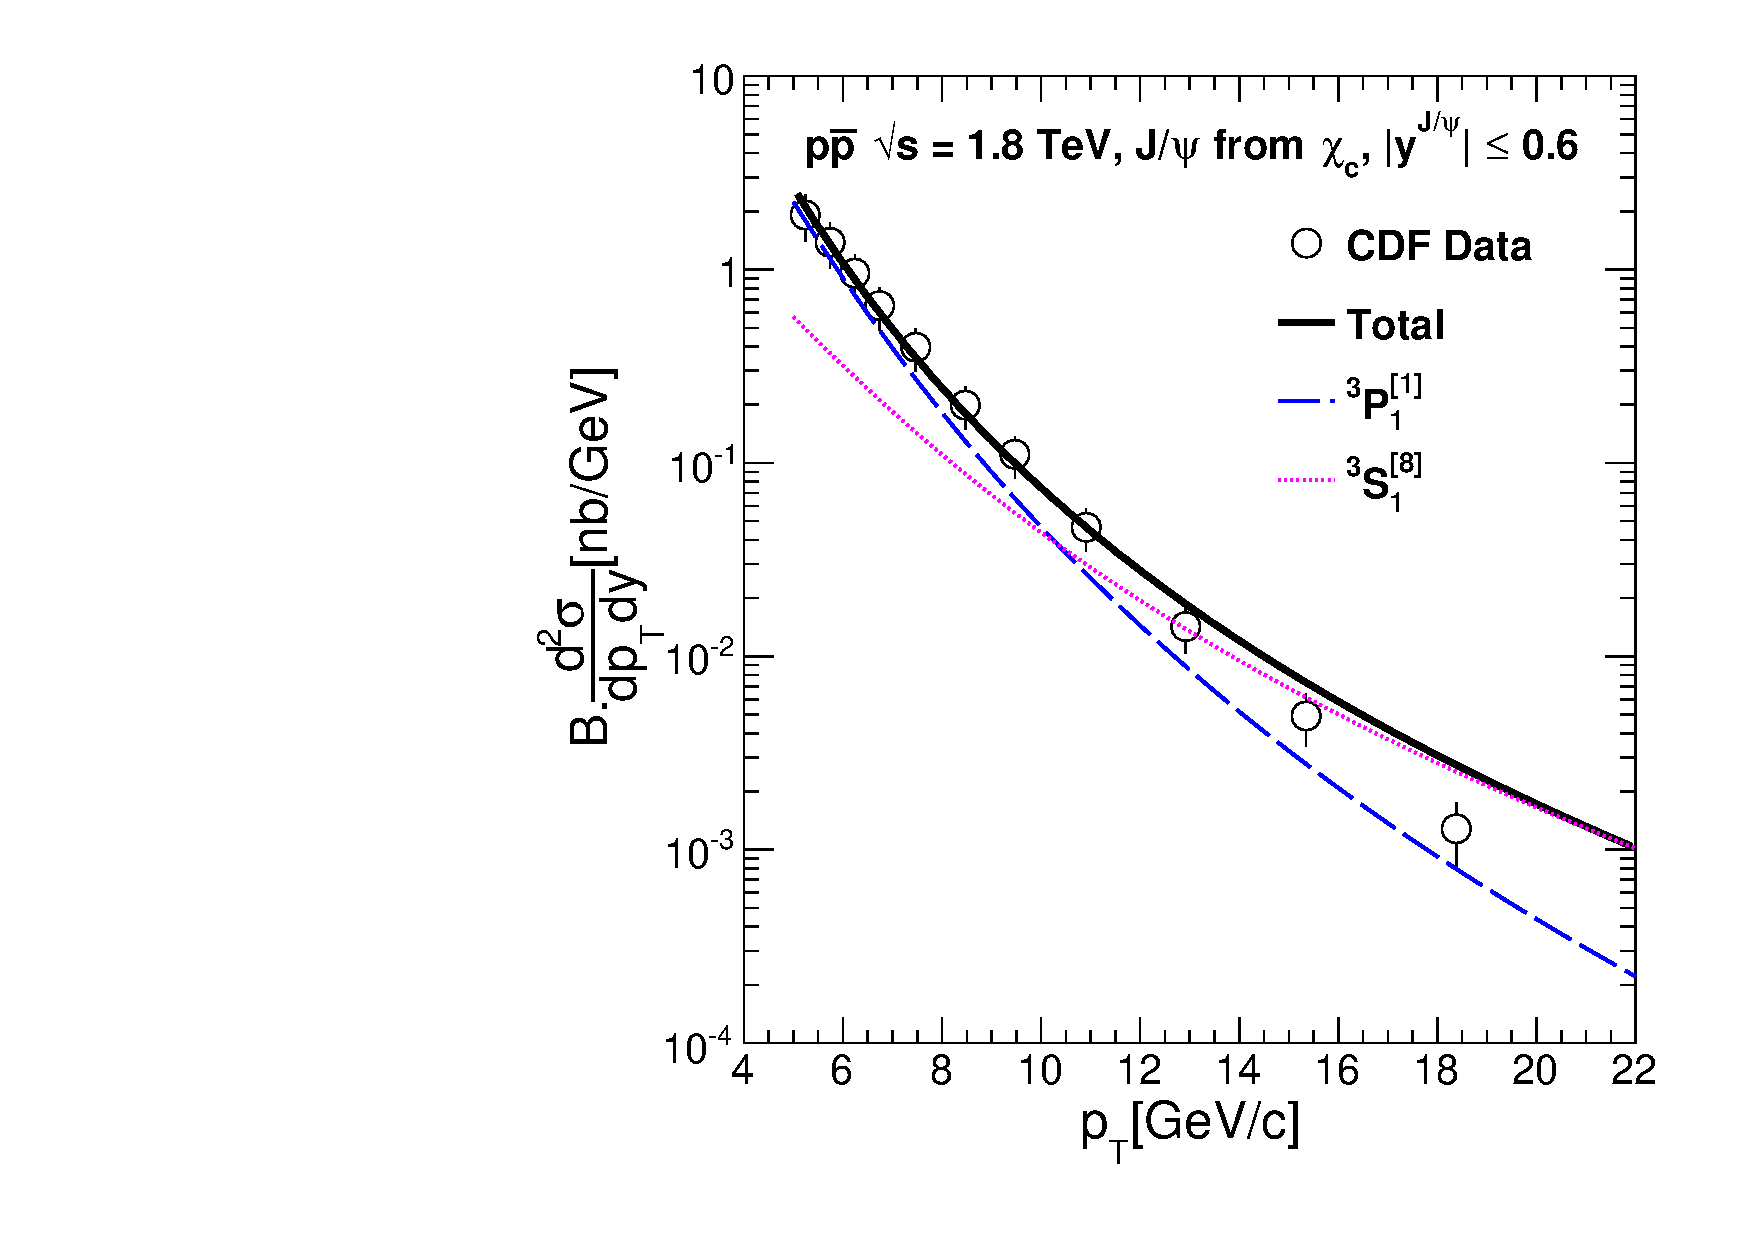
\includegraphics[width=0.49\textwidth]{Figures/Chic/Chic1_CDF_Fit.pdf}
\caption{(Color online) Differential production cross-section of $J/\psi$ from
$\chi_{c1}$ and $\chi_{c2}$ decays as a function of J/$\psi\,\,p_{T}$ measured by CDF experiment at $\sqrt{s}$ = 1.8 TeV~\cite{Abe:1997yz}. 
We use these data sets to constrain color octet LDMEs. Figure also shows our calculations for various components 
of $\chi_{c}$ cross-section.}
\label{Fig:LDMEChicCDF}
\end{figure}
\begin{figure}
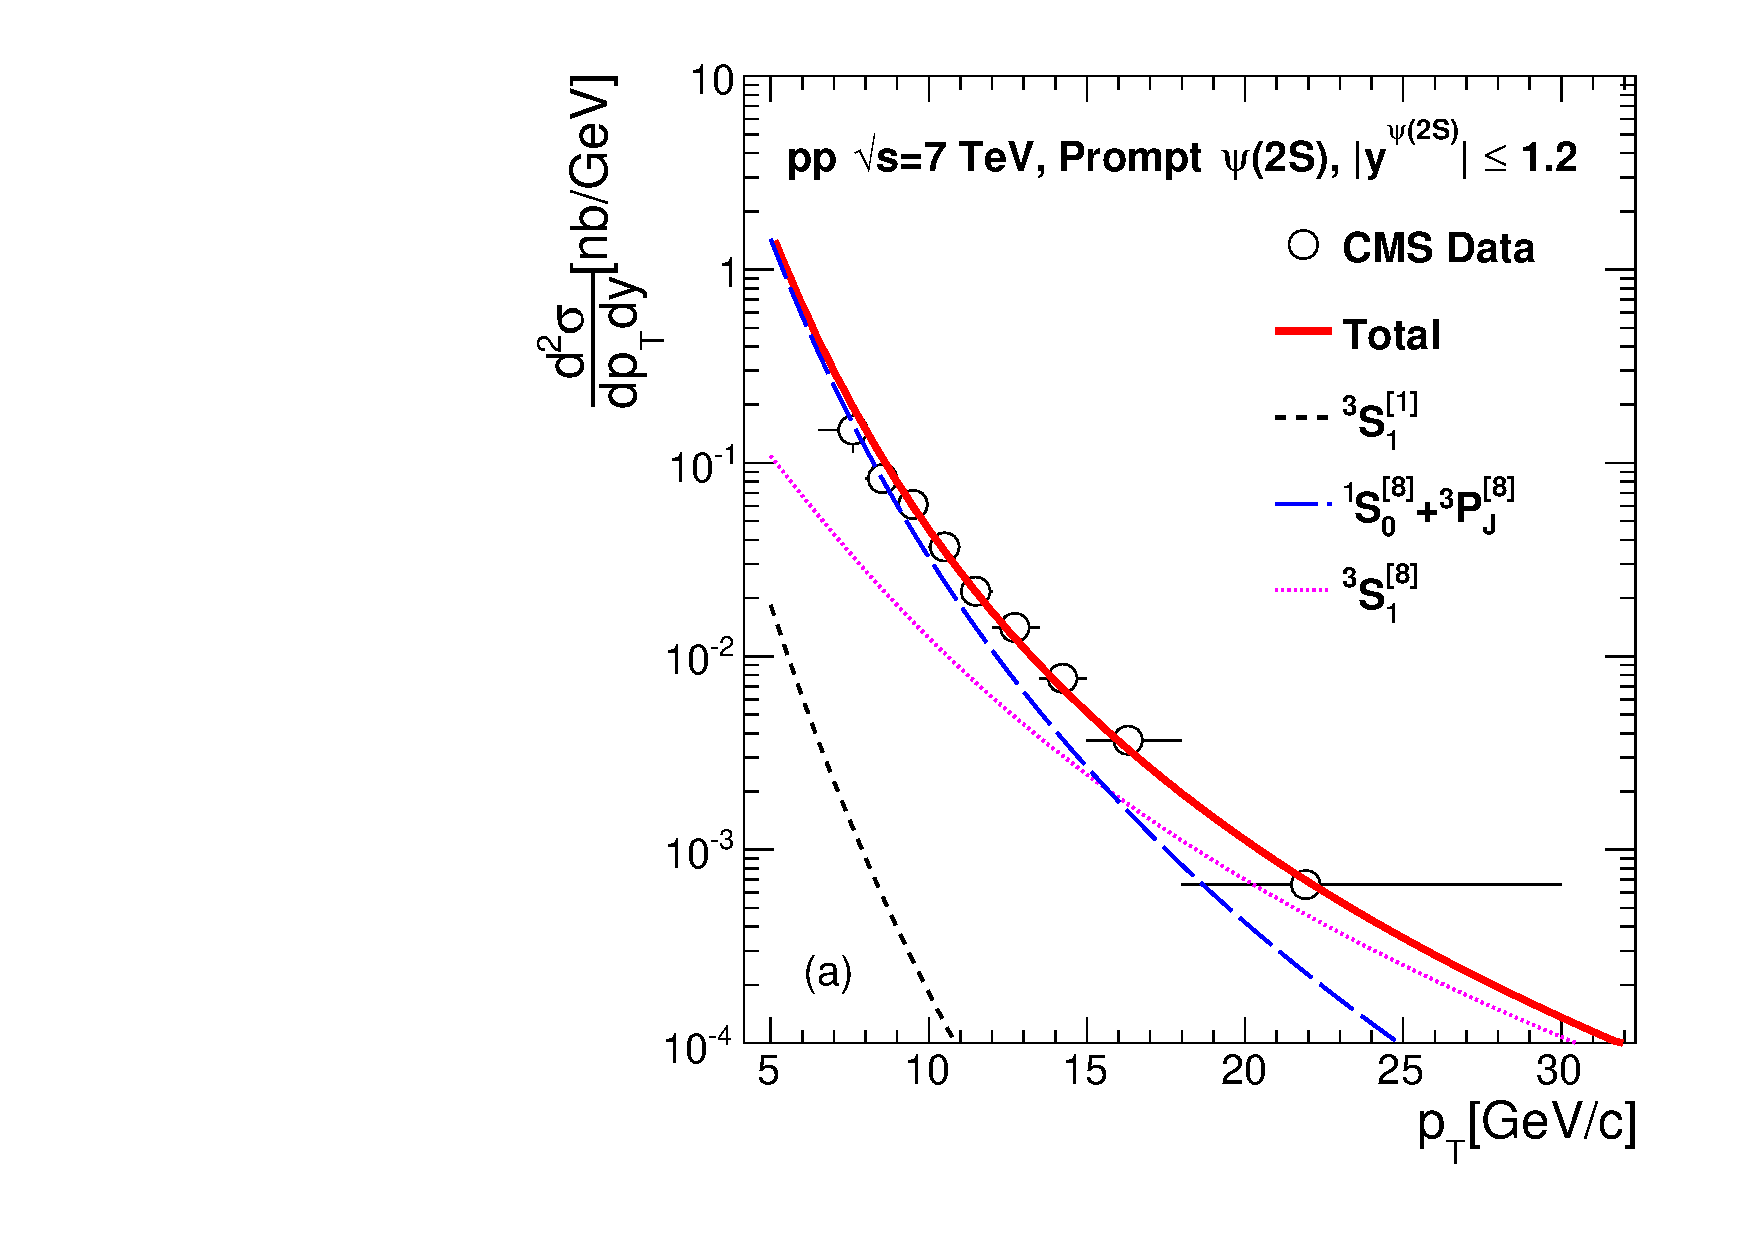
\includegraphics[width=0.49\textwidth]{Figures/Psi2S/Psi2S_CMS_LowPt.pdf}
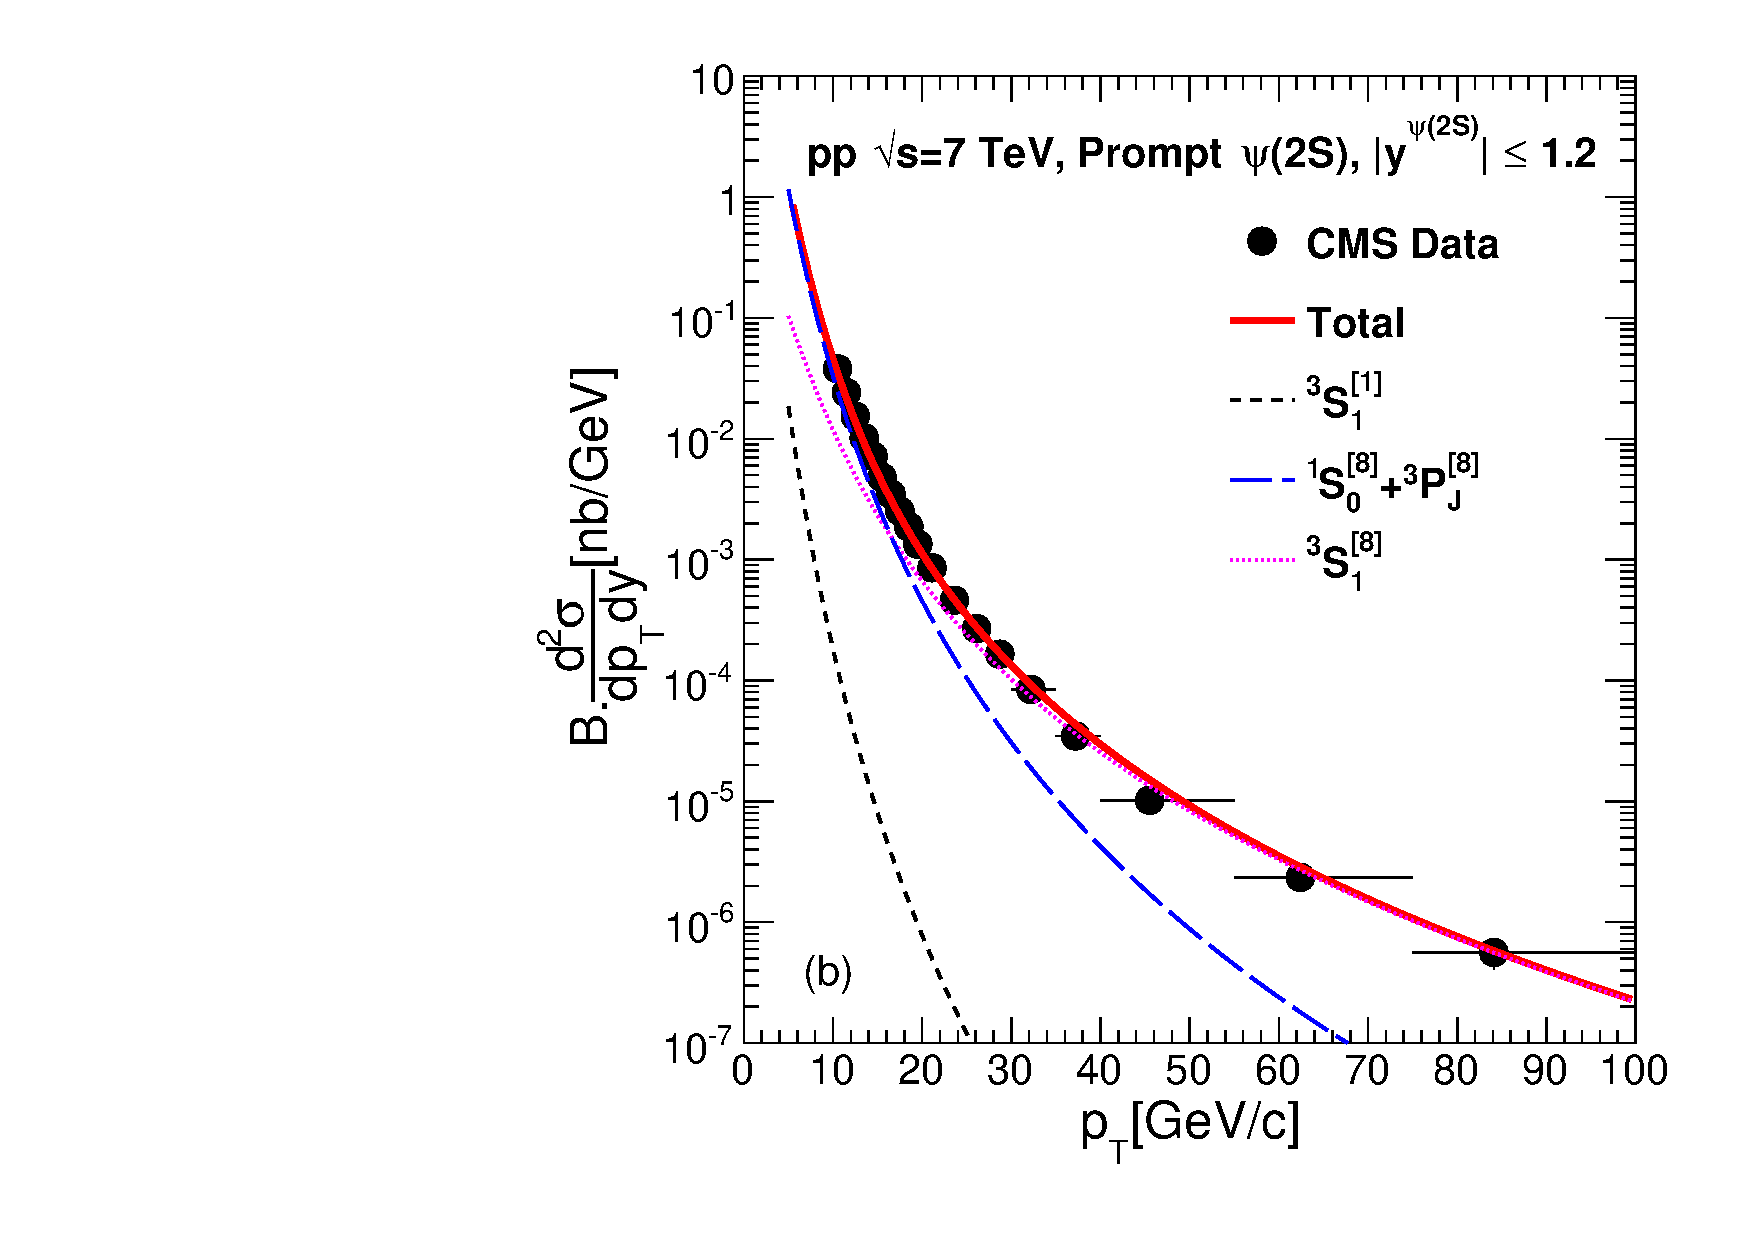
\includegraphics[width=0.49\textwidth]{Figures/Psi2S/Psi2S_CMS_HighPt.pdf}
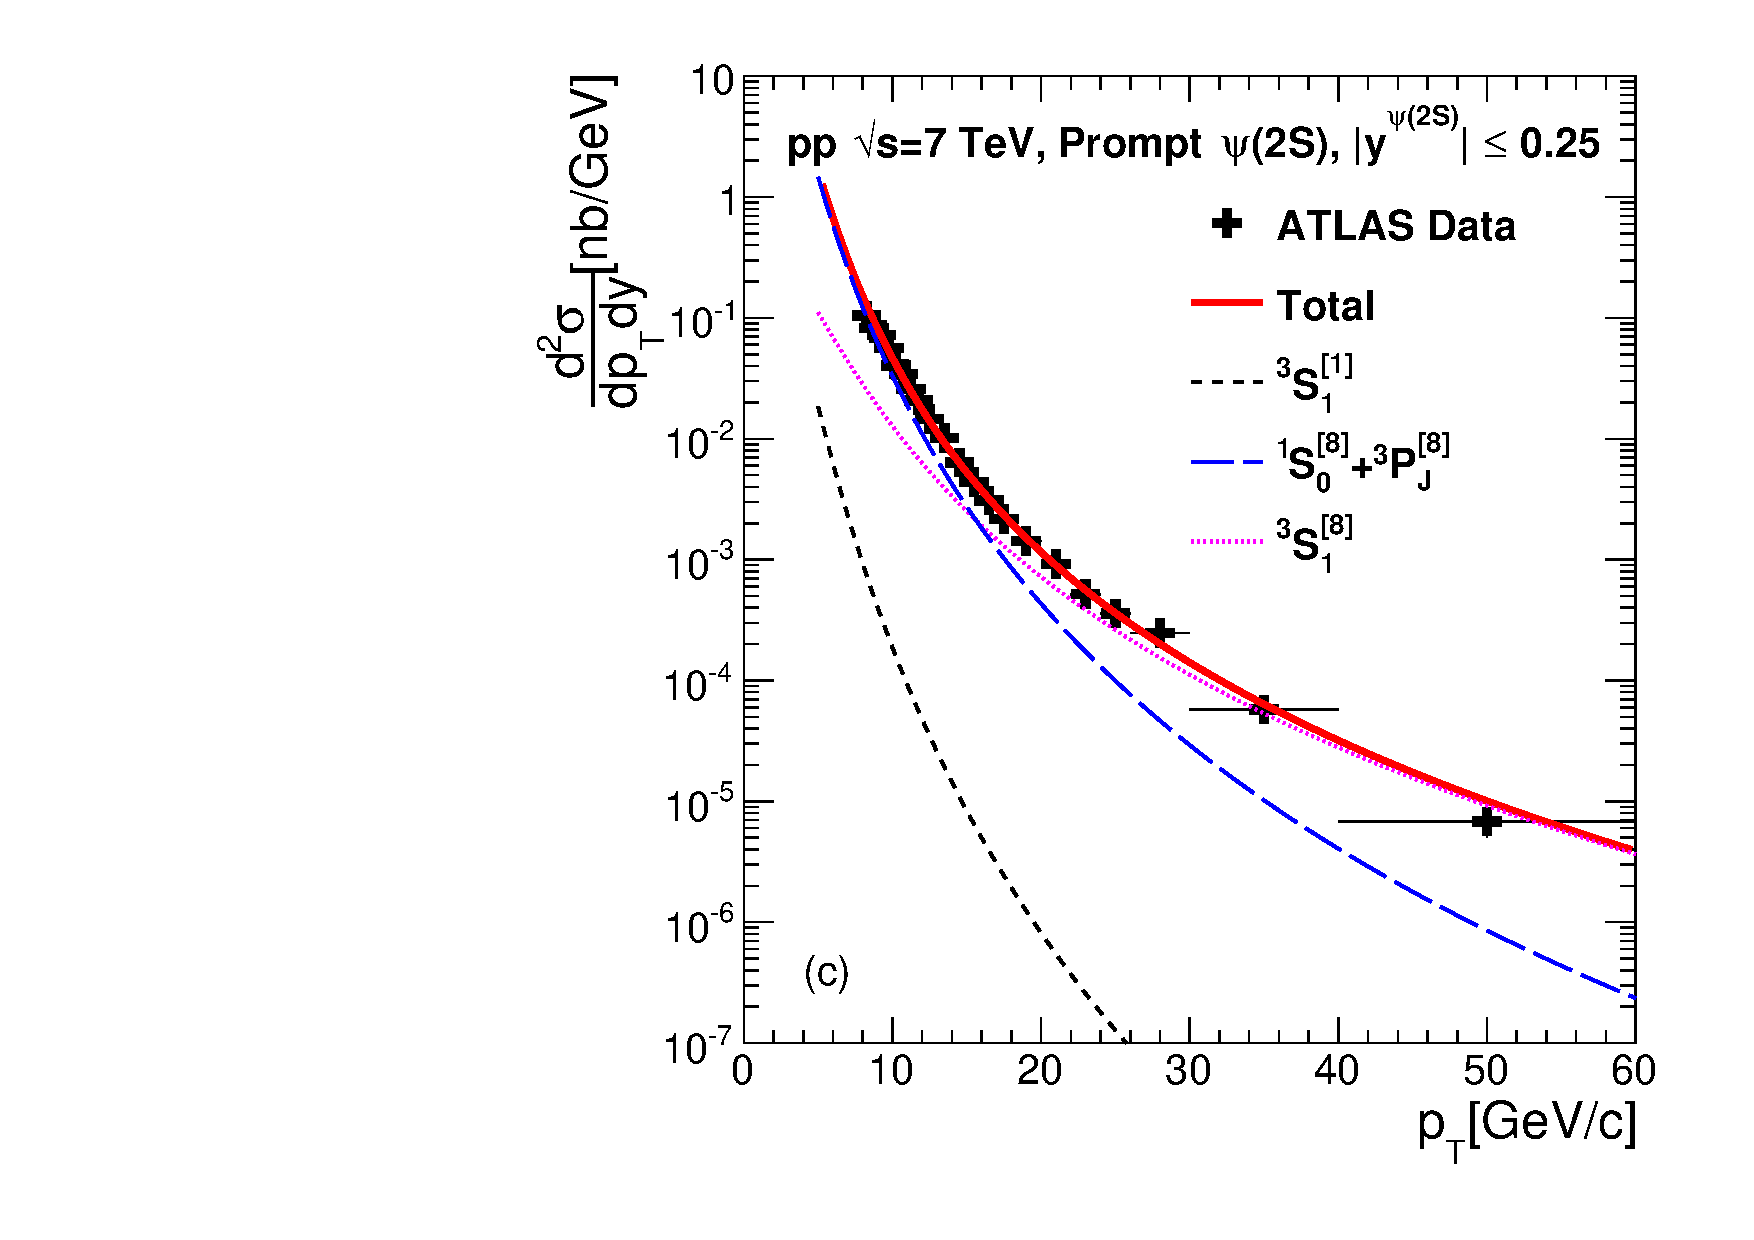
\includegraphics[width=0.49\textwidth]{Figures/Psi2S/Psi2S_ATLAS.pdf}
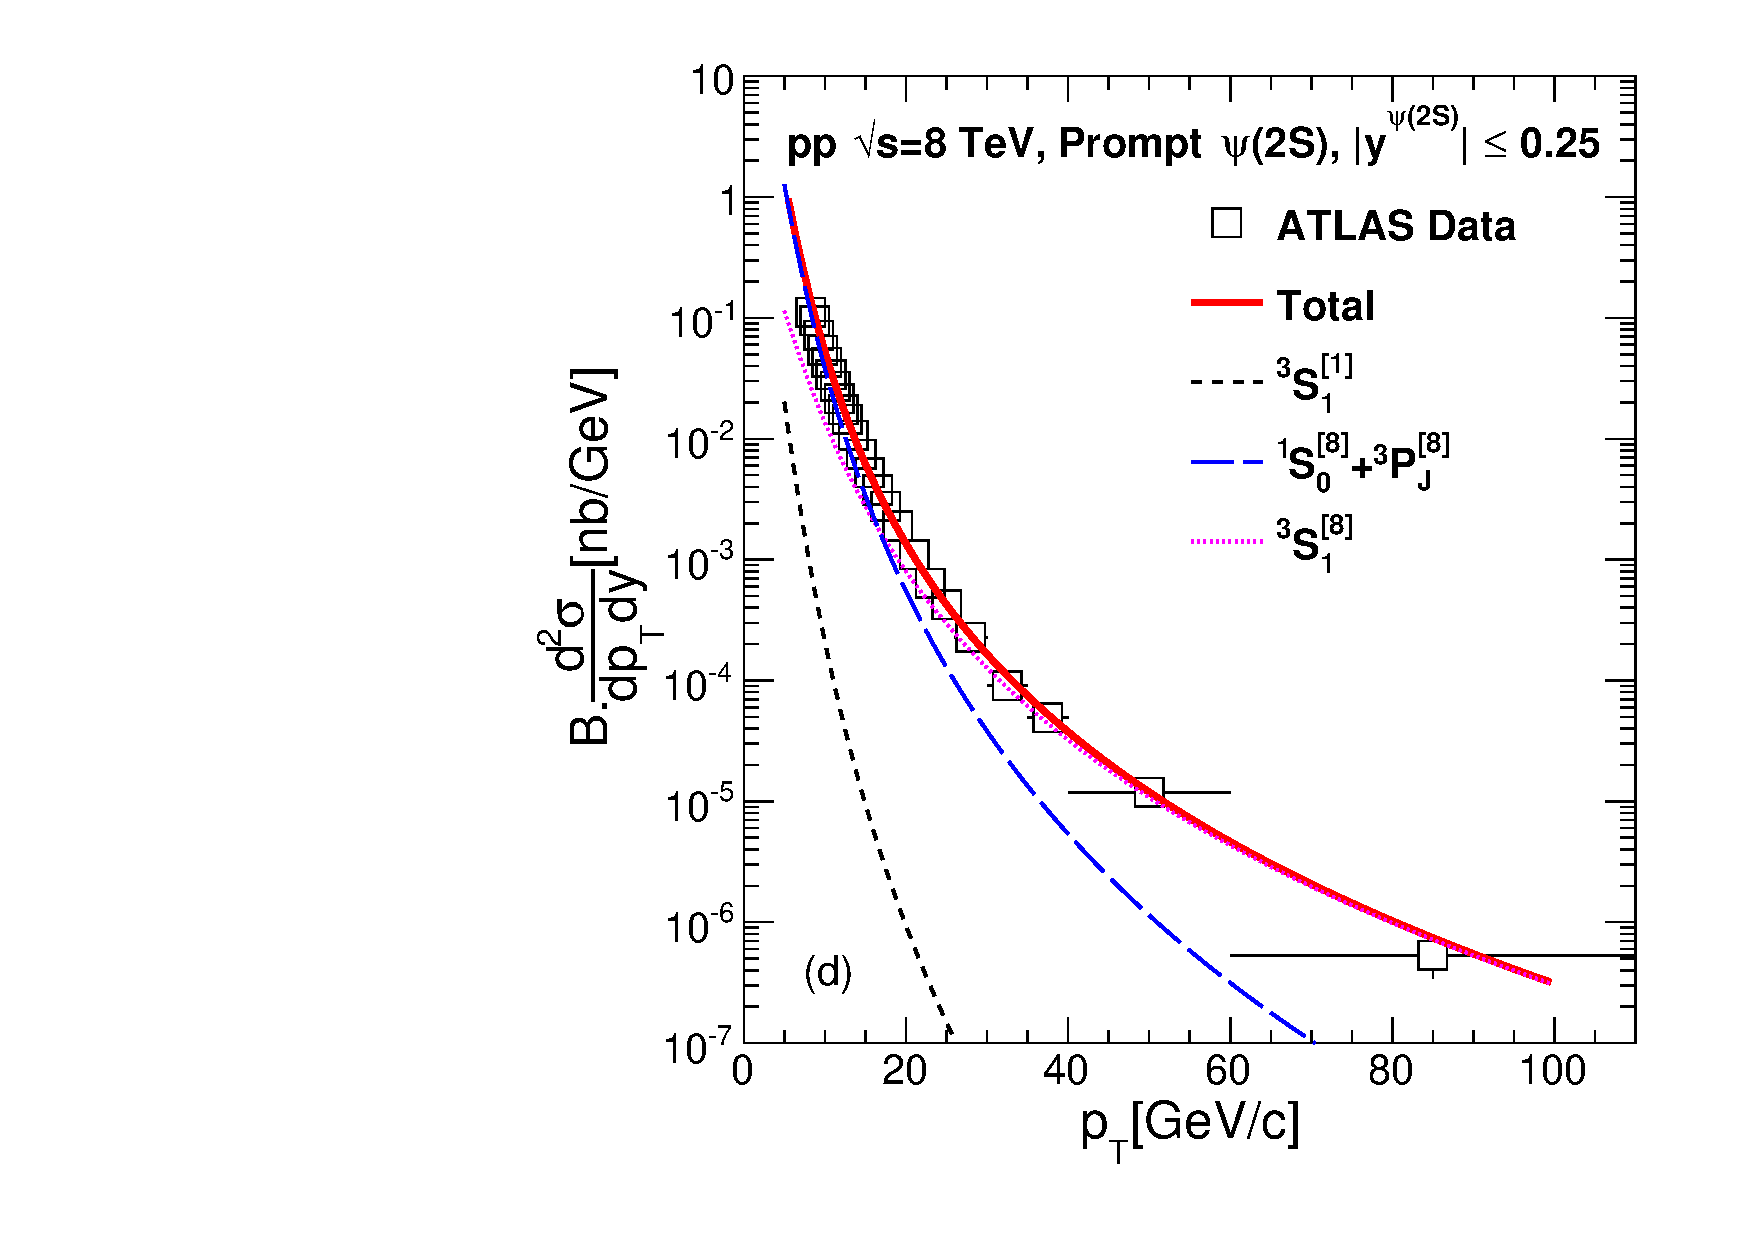
\includegraphics[width=0.49\textwidth]{Figures/Psi2S/Psi2S_ATLAS_8TeV.pdf}
\caption{(Color online) Differential production cross-section of $\psi$(2S) as a function of $p_{T}$ 
collected by LHC experiments at $\sqrt{s}$ = 7 and 8 TeV~\cite{Chatrchyan:2011kc,Khachatryan:2015rra,Aad:2015duc}. 
We use these data sets to constrain color octet LDMEs. Figures also shows our calculations for various components 
of $\psi$(2S) cross-section.}
\label{Fig:LDMEPsi2S}
\end{figure}
\begin{figure}
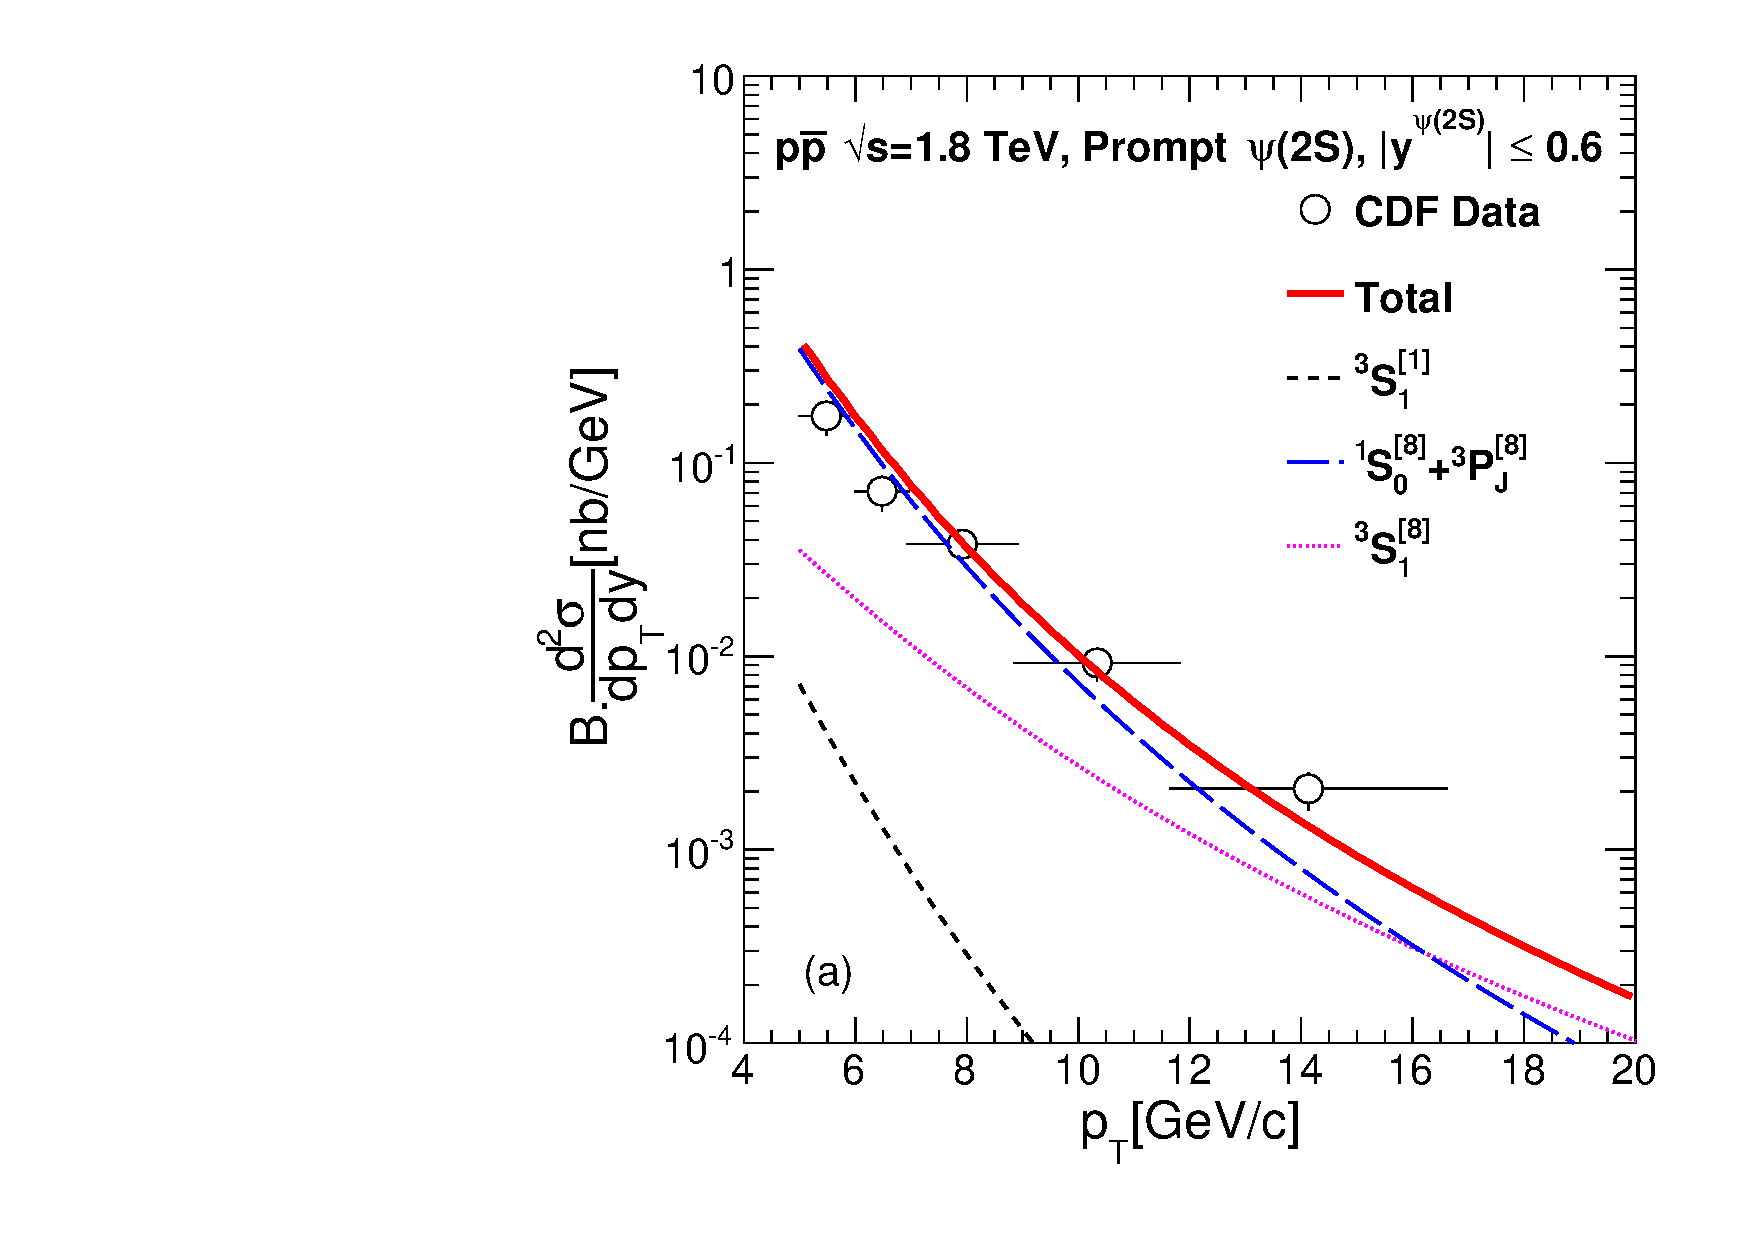
\includegraphics[width=0.49\textwidth]{Figures/Psi2S/Psi2S_CDF_180TeV.pdf}
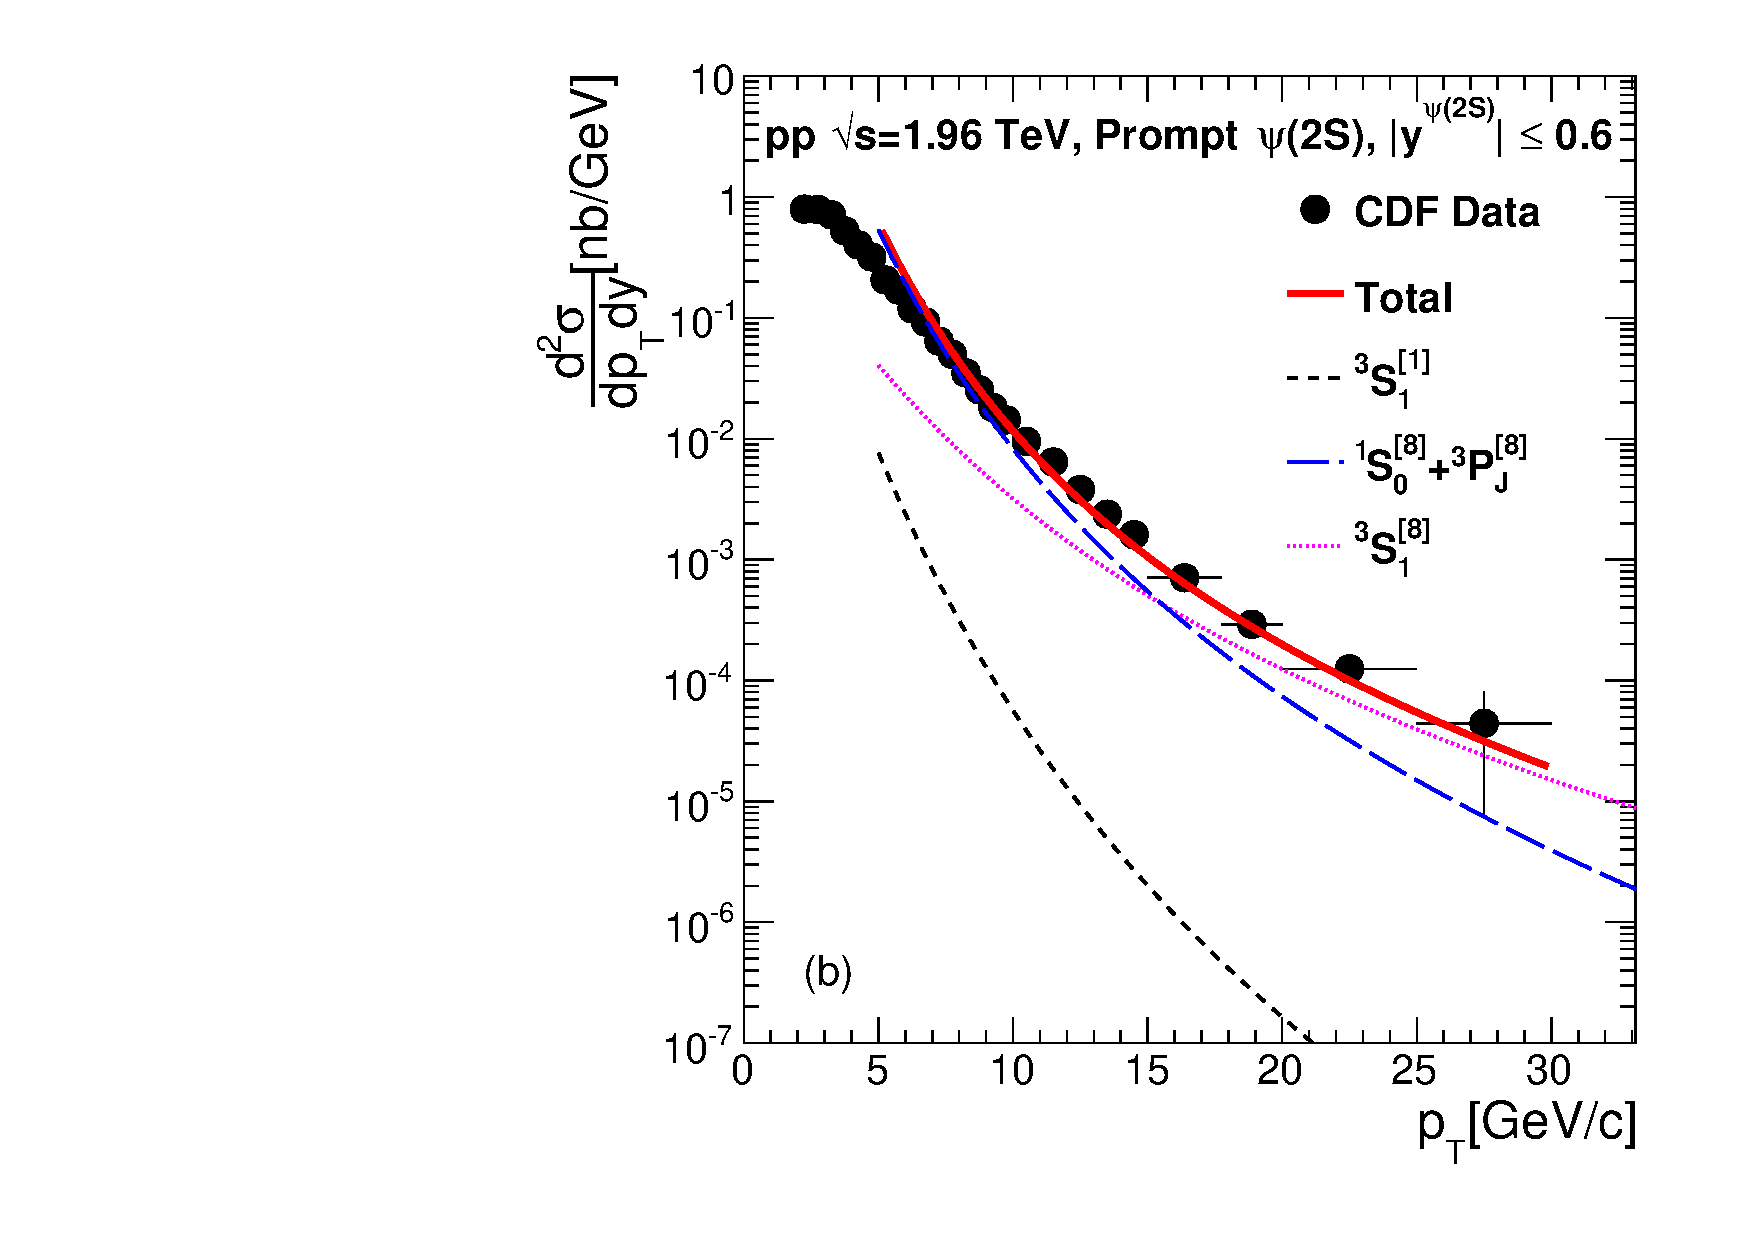
\includegraphics[width=0.49\textwidth]{Figures/Psi2S/Psi2S_CDF_196TeV.pdf}
\caption{(Color online) Differential production cross-section of $\psi$(2S) as a function of $p_{T}$ 
collected by CDF experiment at $\sqrt{s}$ = 1.8 TeV and $\sqrt{s}$ = 1.96 TeV~\cite{Acosta:2004yw}. 
We use these data sets to constrain color octet LDMEs. Figures also shows our calculations for various components 
of $\psi$(2S) cross-section.}
\label{Fig:LDMEPsi2SCDF}
\end{figure}
\begin{figure}
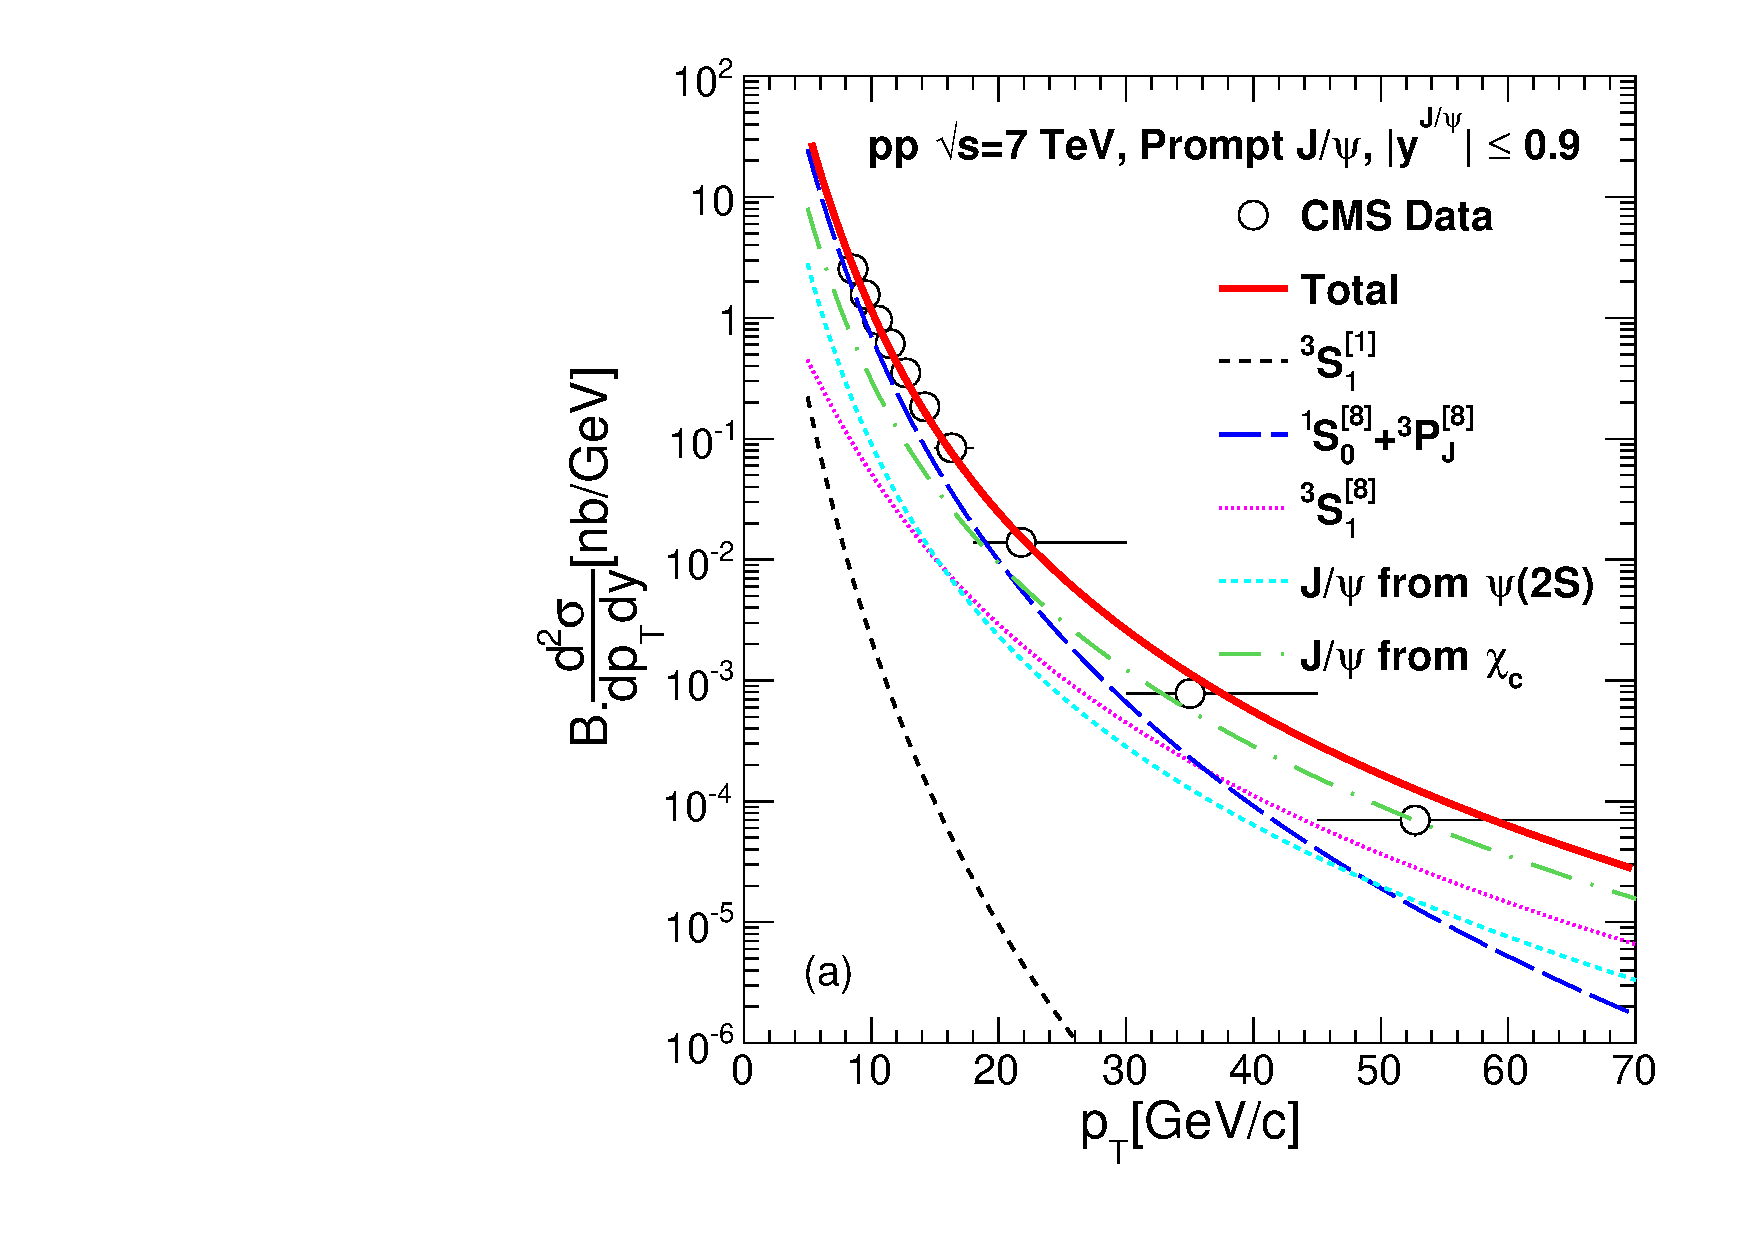
\includegraphics[width=0.49\textwidth]{Figures/JPsi/CMS_New_D2NDPtDy_PromptJPsi_Y0009_Pt.pdf}
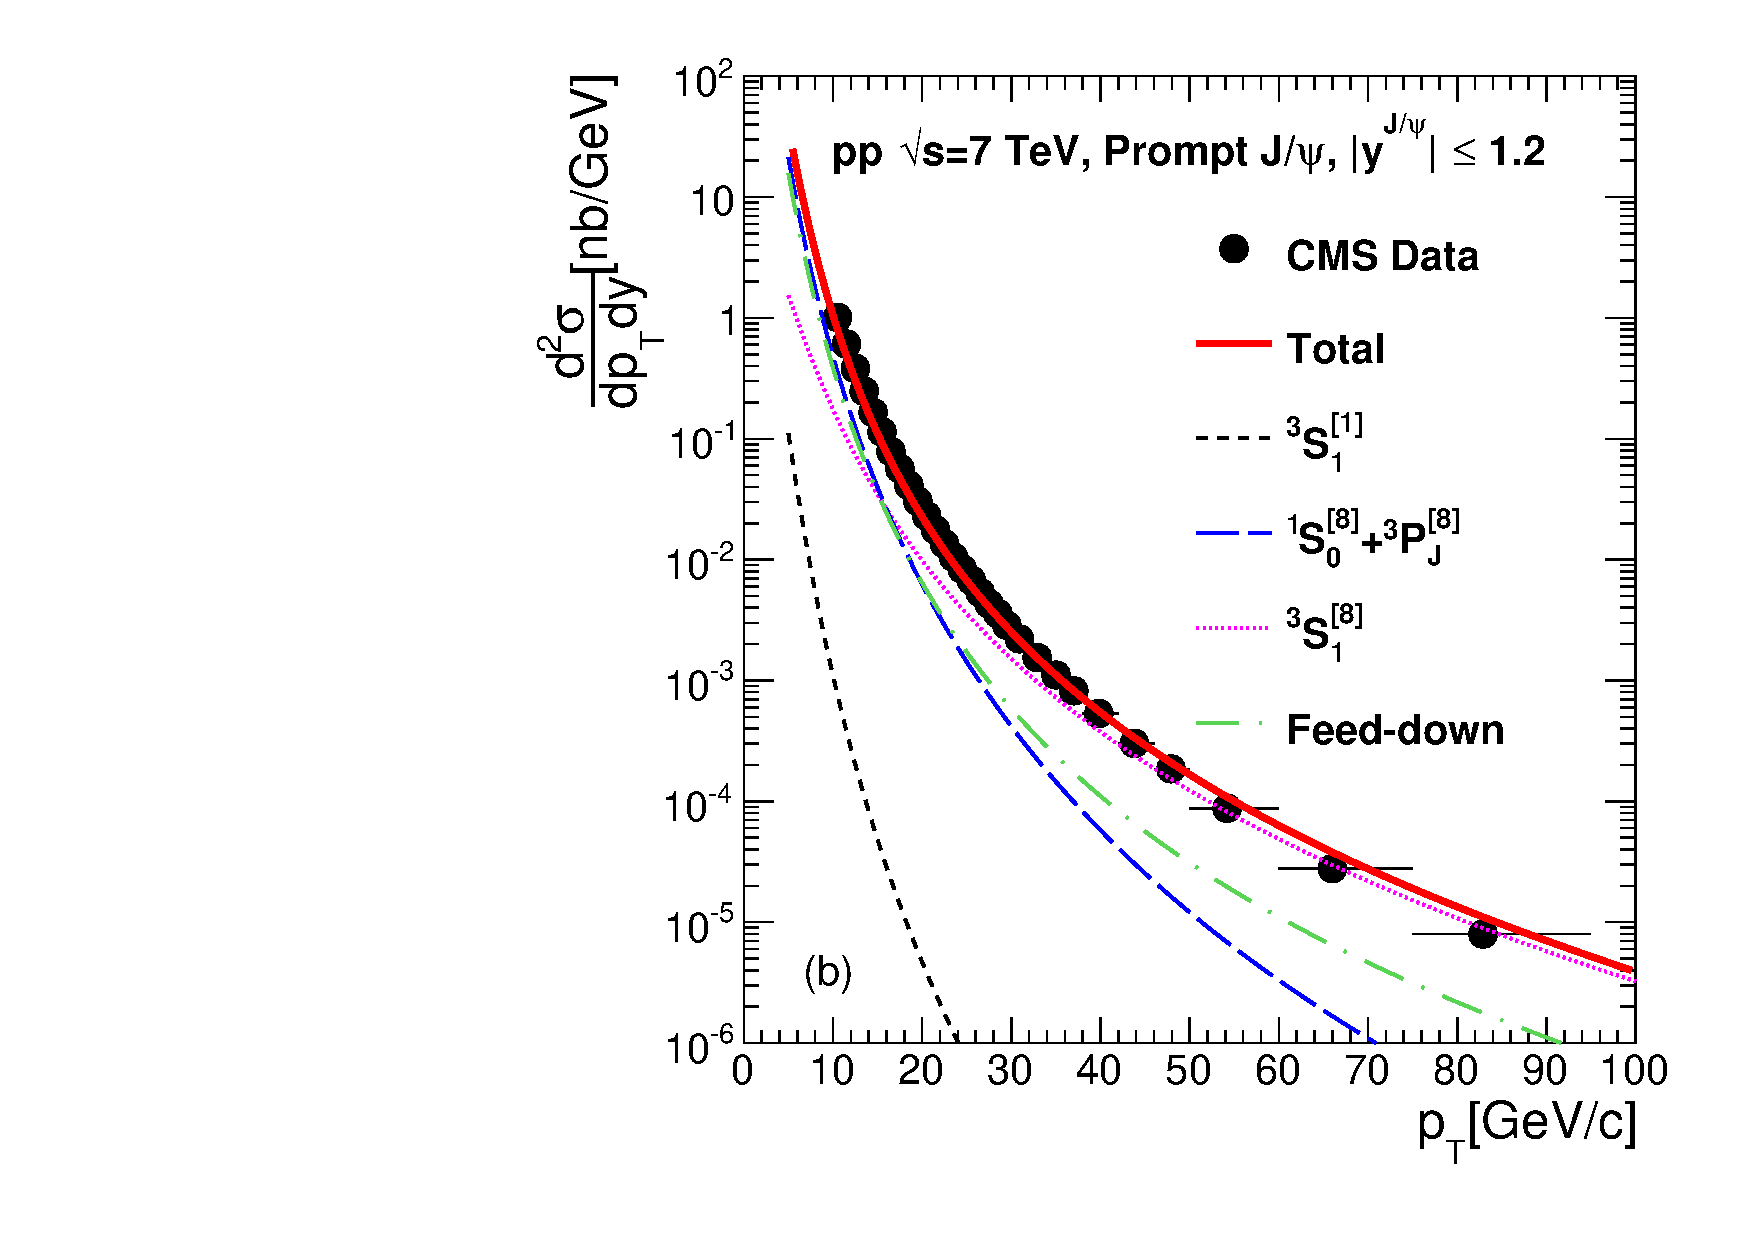
\includegraphics[width=0.49\textwidth]{Figures/JPsi/CMS_Latest_D2NDPtDy_PromptJPsi_Y0012_Pt.pdf}
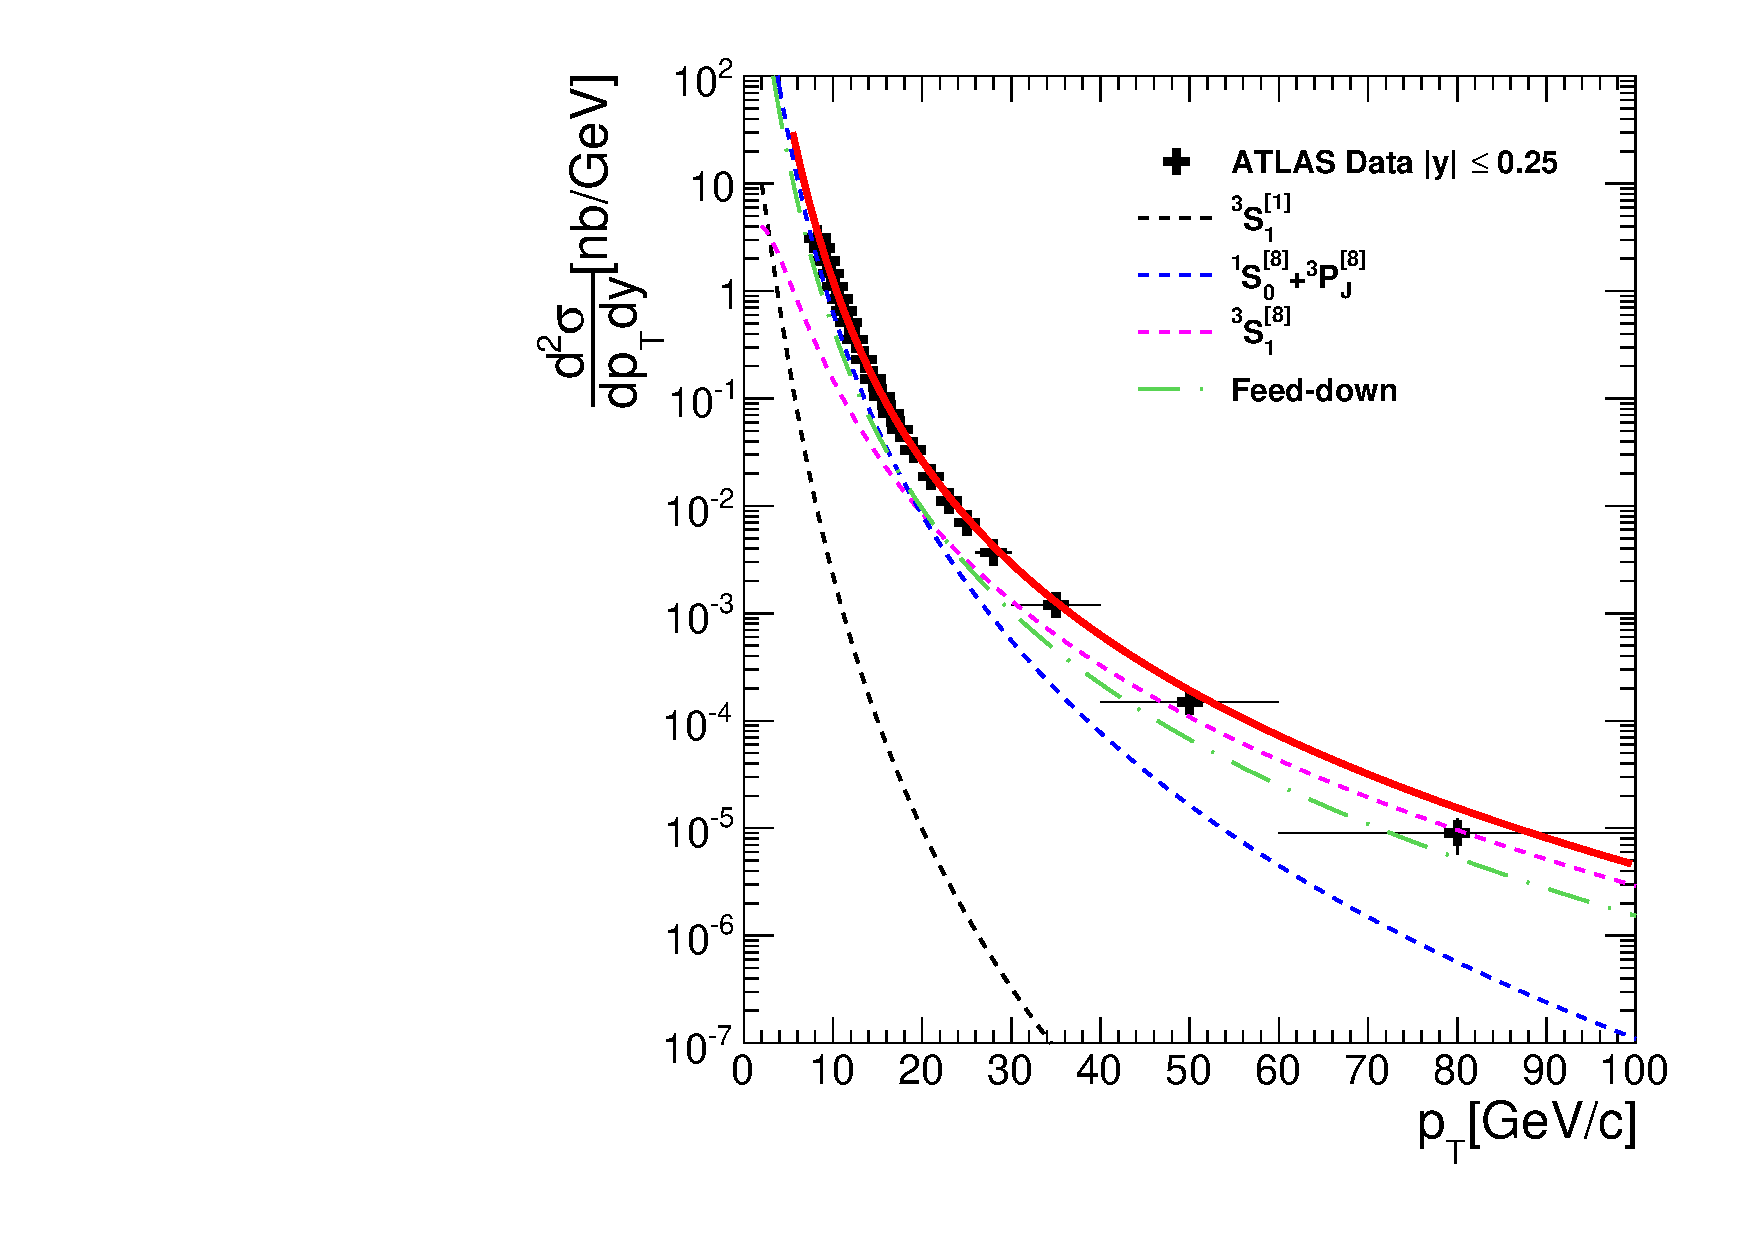
\includegraphics[width=0.49\textwidth]{Figures/JPsi/ATLAS_New_D2NDPtDy_PromptJPsi_Y0025_Pt.pdf}
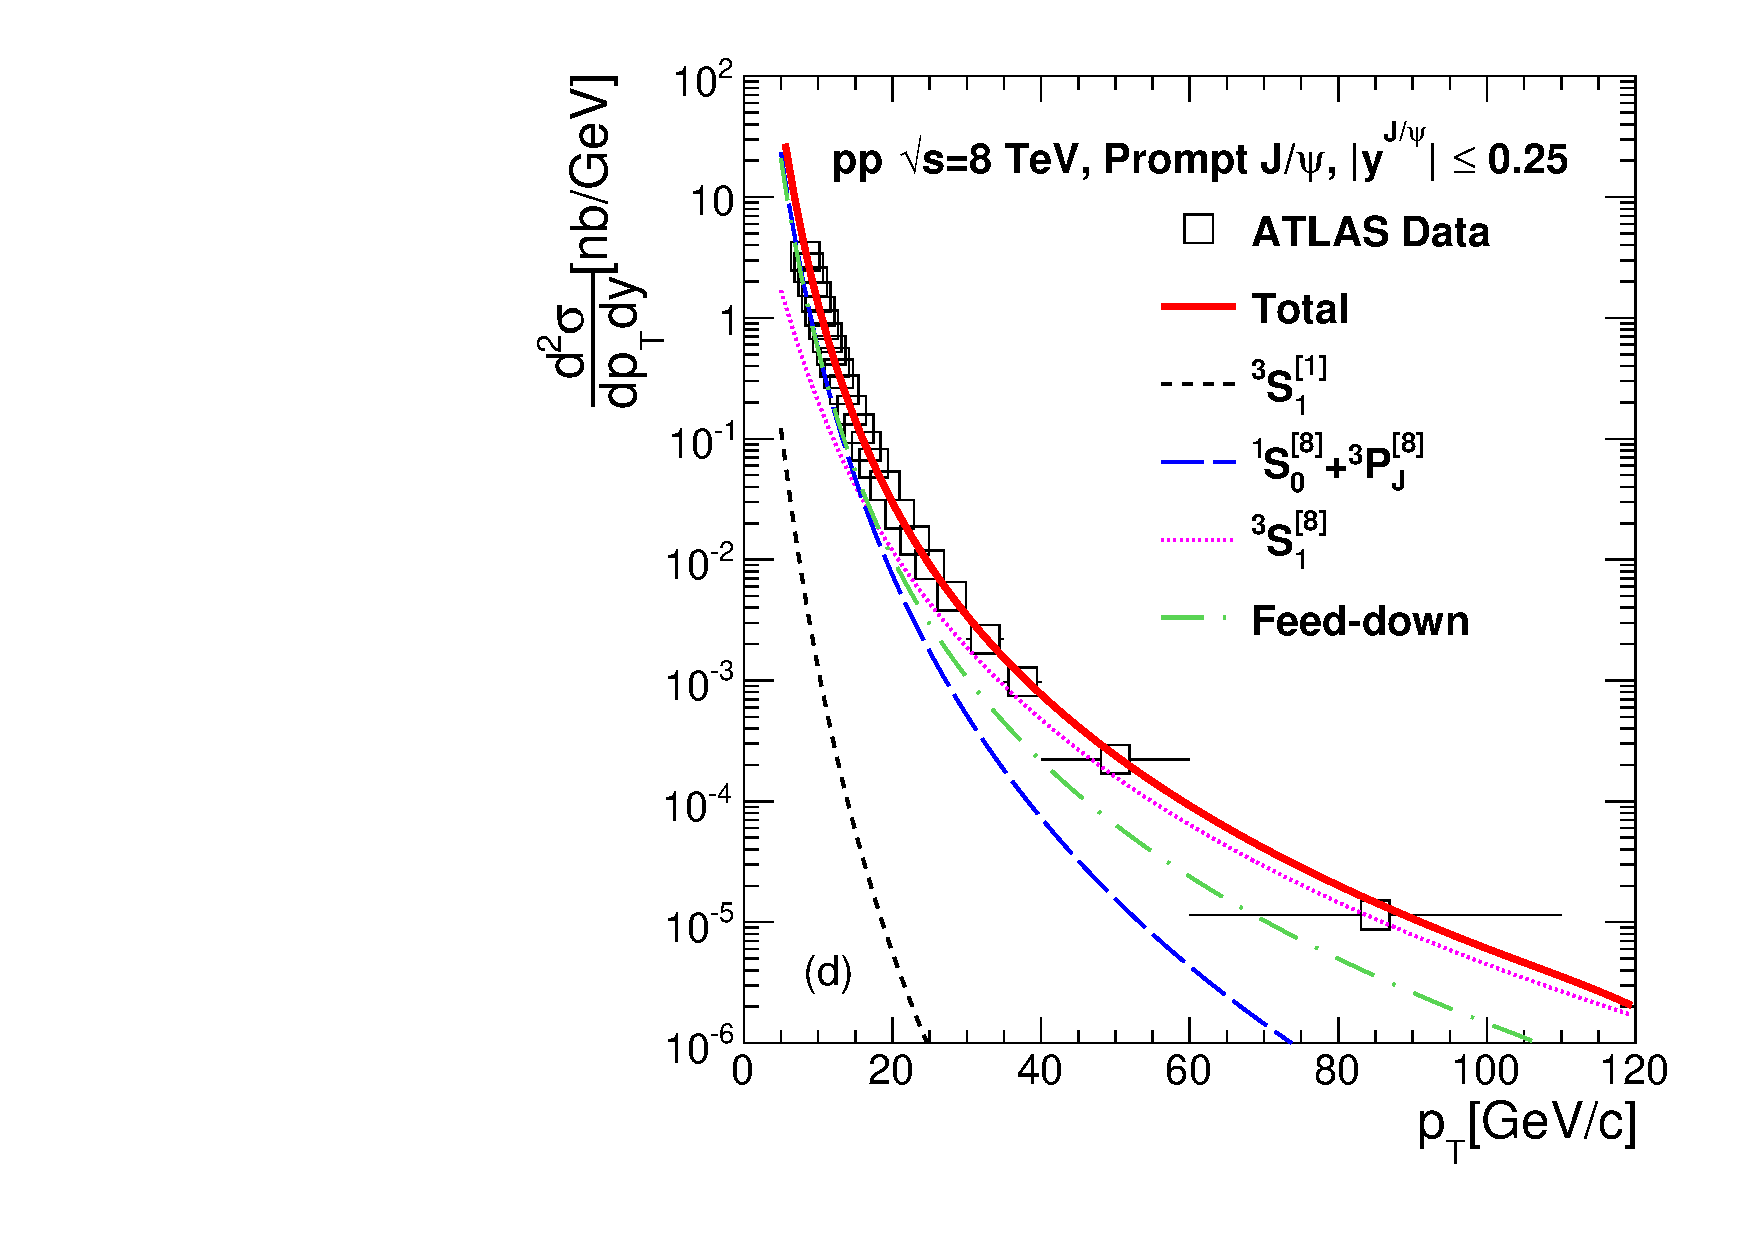
\includegraphics[width=0.49\textwidth]{Figures/JPsi/ATLAS_8TeV_D2NDPtDy_PromptJPsi_Y0025_Pt.pdf}
\caption{(Color online) Differential production cross-section of $J/\psi$ as a function of $p_{T}$ 
collected by LHC experiments at $\sqrt{s}$ = 7 and 8 TeV~\cite{Chatrchyan:2011kc,Khachatryan:2015rra,Aad:2015duc}. 
We use these data sets to constrain color octet LDMEs. Figures also shows our calculations for various components 
of $J/\psi$ cross-section and feed-down contribution from higher charmonia states.}
\label{Fig:LDMEJPsi}
\end{figure}
\begin{figure}
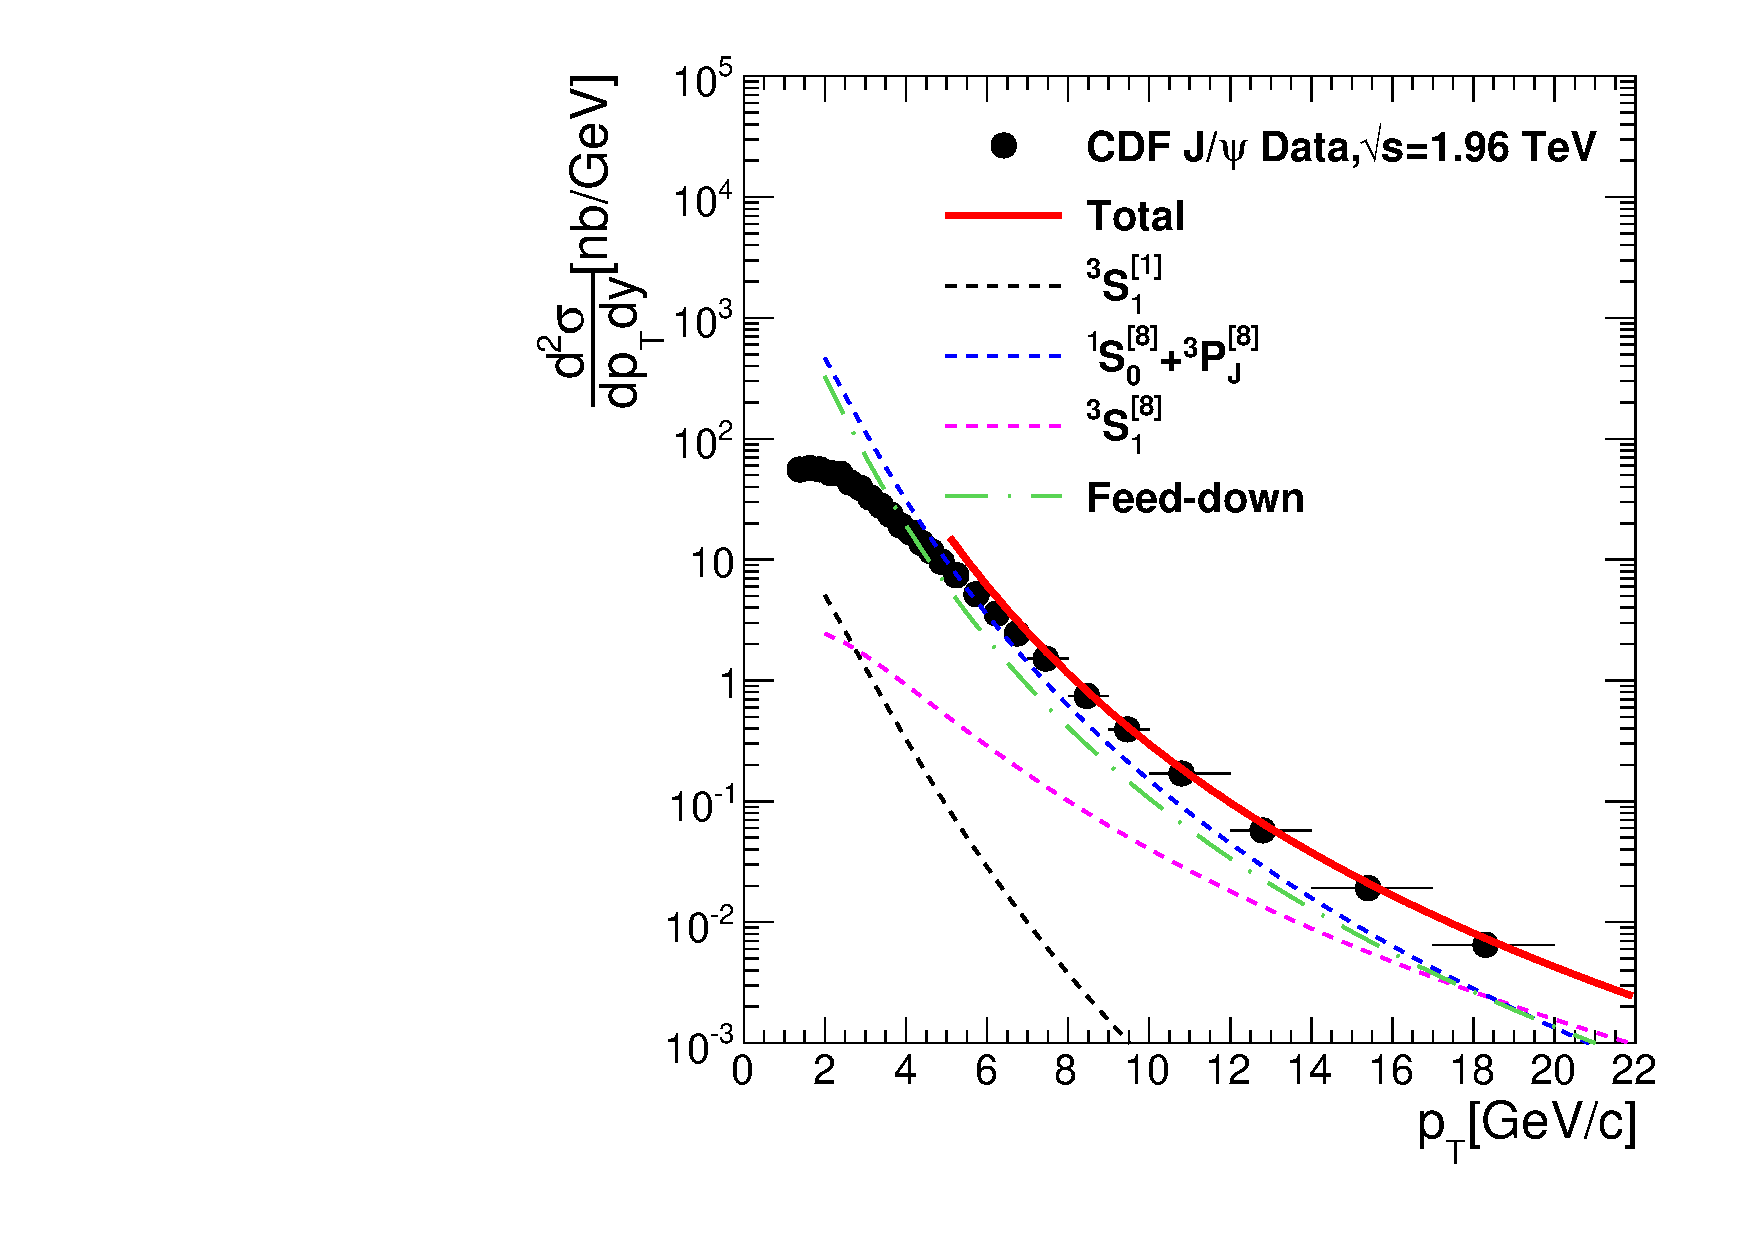
\includegraphics[width=0.49\textwidth]{Figures/JPsi/CDF_196TeV_D2NDPtDy_PromptJPsi_Y0025_Pt.pdf}
\caption{(Color online) Differential production cross-section of $J/\psi$ as a function of $p_{T}$ 
collected by CDF experiment at $\sqrt{s}$ = 1.96 TeV~\cite{Acosta:2004yw}. 
We use these data sets to constrain color octet LDMEs. Figures also shows our calculations for various components 
of $J/\psi$ cross-section and feed-down contribution from higher charmonia states.}
\label{Fig:LDMEJPsiCDF}
\end{figure}
\begin{figure}
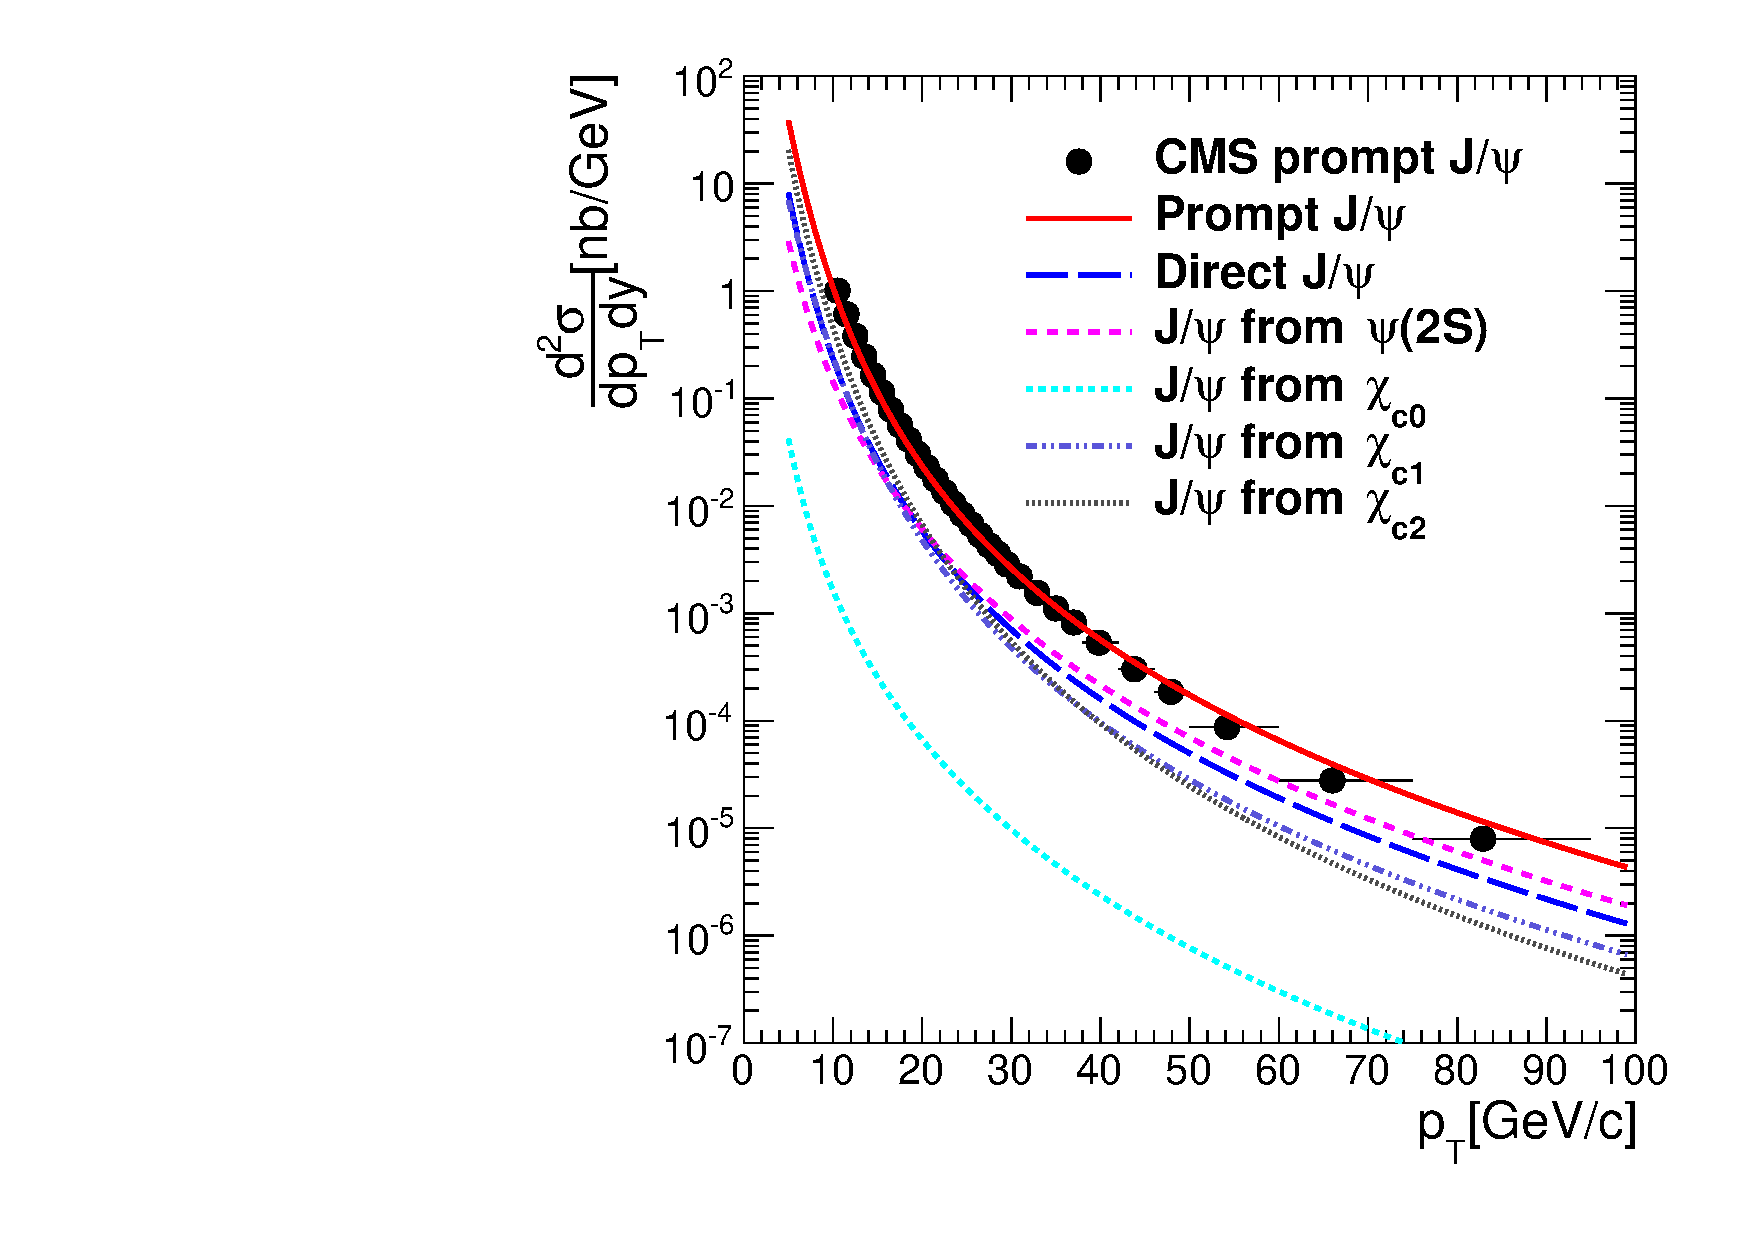
\includegraphics[width=0.49\textwidth]{Fig1a_PromptJPsi_CMS_Y0012_S7TeV.pdf}
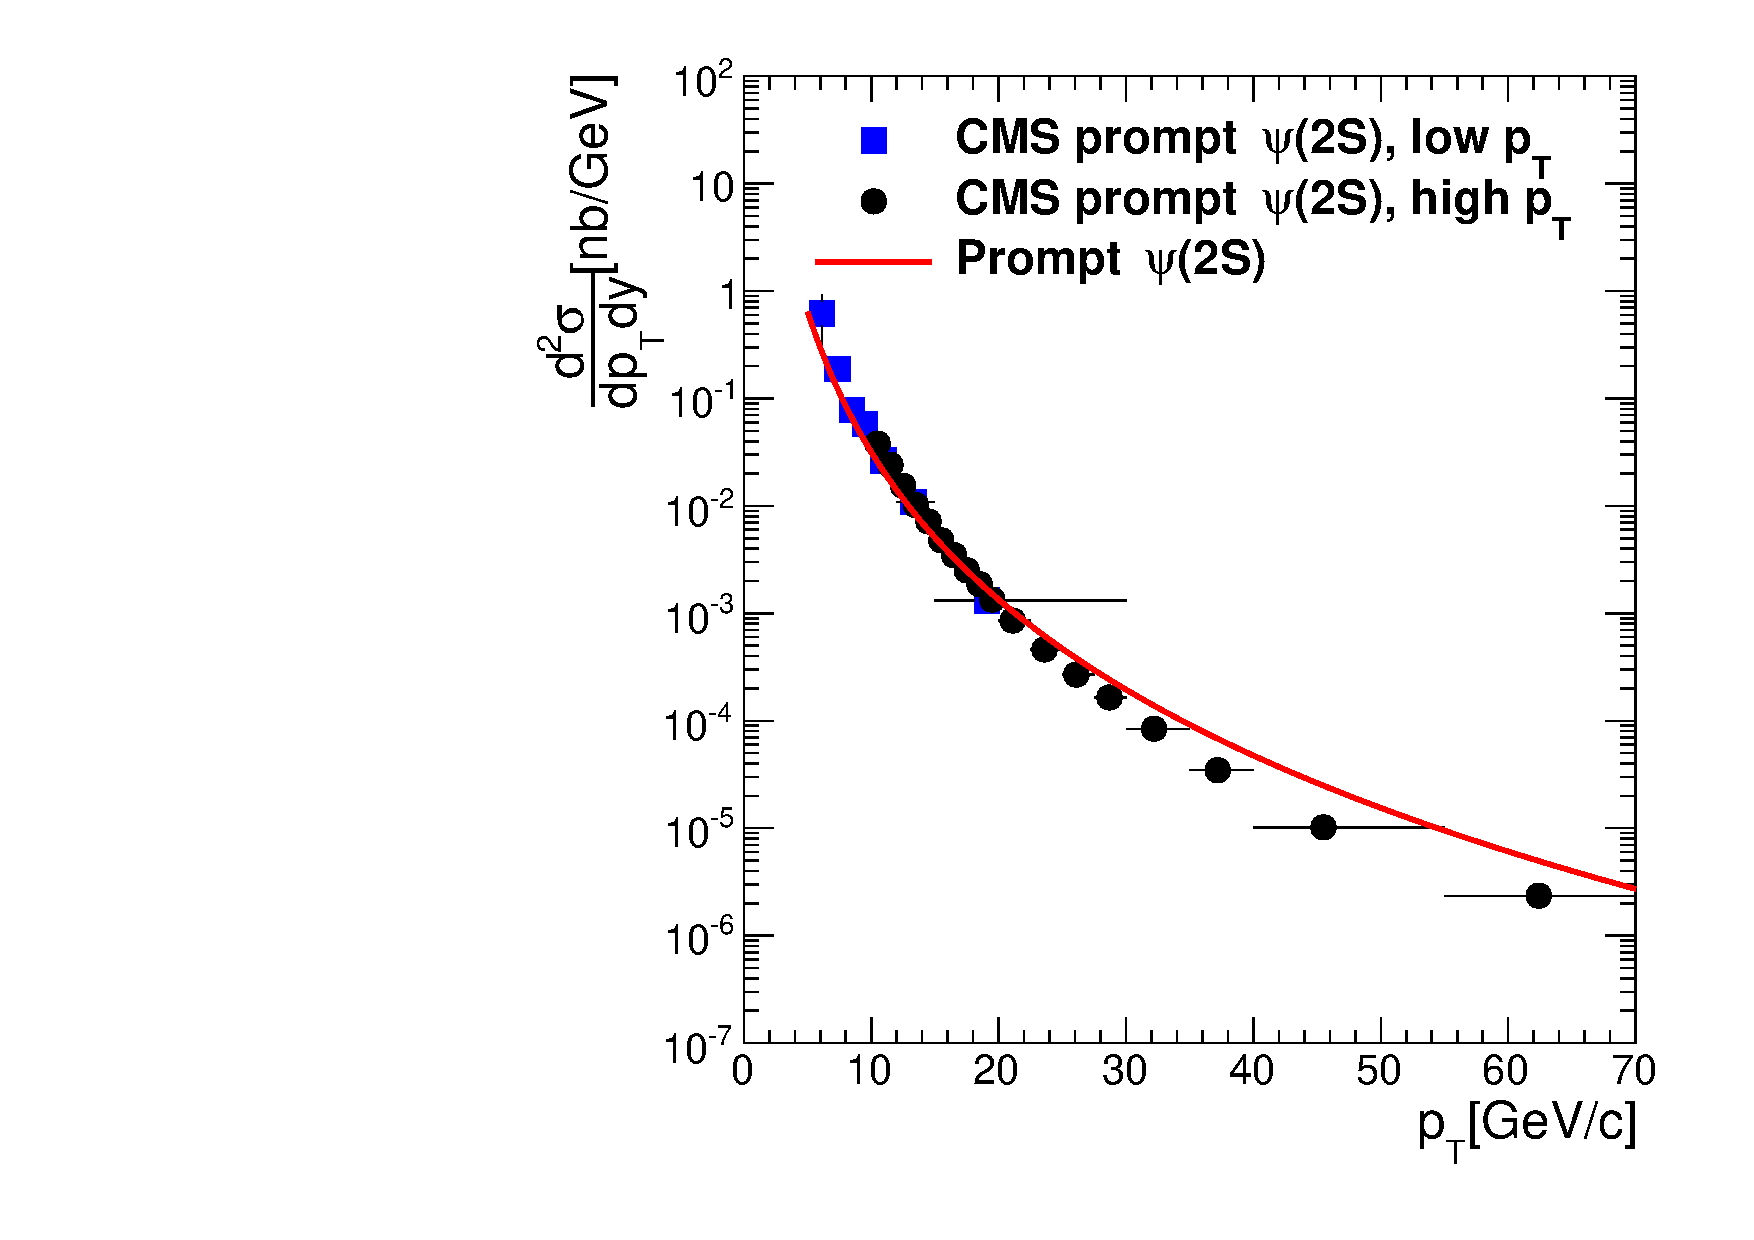
\includegraphics[width=0.49\textwidth]{Fig1b_Psi2S_CMS_Y012_S7TeV.pdf}
\caption{(Color online) Differential production cross-section of $J/\psi$ and $\psi$(2S) as a function of $p_{T}$ compared 
  with the CMS~\cite{Chatrchyan:2011kc,Khachatryan:2015rra} data.}
\label{Fig:SigmaPsi}
\end{figure}
%%%%%%%%%%%%%%%%%%%%%%%%%%%%%%%%%%%%%%%%%%%%%%%%%%%%%%%%%%%%%%%%%%%%%%%%%%%%%%%%%%%%%%%%%%%%%%%%%%%%%%%%%%%%%%%%%%%%%
\section{Result and Discussion}
Figure~\ref{Fig:SigmaPsi} (a) shows the differential production cross-section of 
prompt J/$\psi$ as a function of transeverse momentum ($p_{T}$) compared with the 
CMS measurements~\cite{Khachatryan:2015rra}. We have calculated differential production cross-sections 
for all the relevant resonances. These cross sections are then appropriately scaled with proper branching 
fractions and total cross section for prompt J/$\psi$ is calculated and shown in Fig.~\ref{Fig:SigmaPsi} (a). 
The $\psi$(2S) has largest contribution at high $p_{T}$ while at low $p_{T}$ contribution 
from  $\chi_{c1}$ and $\chi_{c2}$ exceed the $\psi$(2S) contribution. After adding all the contributions, the $p_T$ 
dependence of prompt J/$\psi$ differential production cross-section are described reasonably well by 
our calculations. The $\psi(2S)$ has no significant feed-down contributions from higher mass states. We call this 
direct contribution as "prompt $\psi$(2S)" to be consistent with the J/$\psi$ calculations. 
Figure~\ref{Fig:SigmaPsi}(b) shows the differential production cross-section of prompt $\psi$(2S) as a function 
of $p_{T}$ compared with the CMS measurements~\cite{Khachatryan:2015rra}. Here also our calculations qualitatively
reproduced the mesaured cross section.\\  
{\color{red} Discription for old figures, should put new figures of cross section prediction at 14 TeV
  and describe the fitting figures.}
%%%%%%%%%%%%%%%%%%%%%%%%%%%%%%%%%%%%%%%%%%%%%%%%%%%%%%%%%%%%%%%%%%%%%%%%%%%%%%%%%%%%%%%%%%%%%%%%%%%%%%%%%%%%%%%%%%%%%%
\section{Summary}
We have calculated the differential production cross-section of prompt J/$\psi$ and prompt $\psi$(2S)
as a function of transverse momentum. For the J/$\psi$ meson all the relevent contributions 
from higher mass states are estimated. The $\psi$(2S) meson does not have significant contributions
from higher mass states. The calculations for  prompt J/$\psi$ and prompt $\psi$(2S) are compared with
the measured data at LHC. A fairly good agreement between measured data and calculations is observed
in low $p_{T}$ range. The reevaluation of LDME is in progress using latest data from LHC to achieve good
description of data in the whole $p_{T}$ range. 
\newpage
\appendix
%\begin{appendices}
\section{Short distance pQCD cross sections for quarkonia production}
\label{section:pqcd}
Here we list the lowest order QCD cross sections for the resonance production used 
in our calculations. We write the formulas in terms of the invariants $\cs$,$\ct$,$\cu$.
where $\cs^2 + \ct^2 + \cu^2 = M^2$ and $M$ is the mass of the resonance considered.
%These parton level invariants are related with the rapidity,y 
%and transeverse momentum $p_{T}$ of the resonance with following relations
%\begin{equation}
%\begin{split}
%\cs = \,&x_{a}\,x_{b}\,s \\
%\ct = \,&M^{2} - x_{a}\,\sqrt{s}\,m_{T}\,e^{-y}\\
%\cu = \,&M^{2} - x_{b}\,\sqrt{s}\,m_{T}\,e^{y}\\
%\end{split}  
%\end{equation}
The subprocesses of resonance production can be
grouped as follows.
To order $\alpha_{s}^{2}$ one only has the
gluon fusion processes, g g $\rightarrow ^{(2S+1)}L_{J}$. This 
process gives resonance with very small $\pT$, so we do not 
use these cross-sections in our calculations.

To order $\alpha_{s}^{3}$, on the other hand, one has typically
two-by-two scattering processes. The relevant cross
sections are given below:

\subsubsection{\bf Color Singlet PQCD cross sections}
\begin{itemize}
\item g q $\rightarrow {\rm ^{(2S+1)}L_{J}}$ q or (q$\rightarrow \bar{\rm q})$
\begin{equation}
\begin{split}
\frac{d\sigma}{d\ct}(^1S_0) = &\frac{2\pi\alphas^{3} (R_{0})^{2}}{9M\cs^2}\cdot\frac{(\ct-M^2)^{2}-2\cs\cu}{(-\ct)(\ct-M^2)^{2}}\\
\frac{d\sigma}{d\ct}(^3P_0) = &\frac{8\pi\alphas^3 (R_{1}^\prime)^{2}}{9M^{3}\cs^2}\cdot\frac{(\ct-3M^2)^{2}(\cs^2+\cu^2)}{(-\ct)(\ct-M^2)^{4}}\\
\frac{d\sigma}{d\ct}(^3P_1) = &\frac{16\pi\alphas^3 (R_{1}^\prime)^{2}}{3M^{3}\cs^2}\cdot\frac{-\ct(\cs^2+\cu^2)-4M^2\cs\cu}{(\ct-M^2)^{4}}\\
\frac{d\sigma}{d\ct}(^3P_2) = &\frac{16\pi\alphas^3 (R_{1}^\prime)^{2}}{9M^{3}\cs^2} \cdot \\
                              &\frac{(\ct-M^2)^2(\ct^2+6M^4)-2\cs\cu(\ct^2-6M^2(\ct-M^2))}{(-\ct)(\ct-M^2)^4}\\
\end{split}  
\end{equation}
\item q $\bar{\rm q}$ $\rightarrow {\rm ^{(2S+1)}L_{J}}$ g
\begin{equation}
\frac{d\sigma}{d\ct}({\rm ^{(2S+1)}L_{J}})=-\frac{8}{3}\frac{\ct^2}{\cs^2}\frac{d\sigma}{d\ct}({\rm g q \rightarrow ^{(2S+1)}L_{J} q})|_{\ct\leftrightarrow\cu}
\end{equation}
\item g g $\rightarrow {\rm ^{(2S+1)}L_{J}}$ g
\begin{equation}
\begin{split}
\frac{d\sigma}{d\ct}(^3S_1) = &\frac{5\pi\alphas^{3} (R_{0})^{2}}{9M\cs^2}\cdot \frac{M^2}{(\cs-M^2)^2 (\ct-M^2)^2 (\cu-M^2)^2}\\
                             &\cdot \{[\cs^2(\cs-M^2)^2]+[\cs\rightarrow\ct]+[\cs\rightarrow\cu] \}\\
\frac{d\sigma}{d\ct}(^1S_0) = &\frac{\pi\alphas^{3} (R_{0})^{2}}{2M\cs^2}\frac{1}{\cs\ct\cu(\cs-M^2)^2(\ct-M^2)^2(\cu-M^2)^2}\\
                              &\cdot\{[\cs^4(\cs-M^2)^2((\cs-M^2)^2+2M^4)\\
                              &-\frac{4}{3}\cs\ct\cu(\cs^2+\ct^2+\cu^2)(\cs-M^2)(\ct-M^2)(\cu-M^2)\\
                              &+\frac{16}{3}M^2\cs\ct\cu(\cs^2\ct^2+\cs^2\cu^2+\ct^2\cu^2)\\
                              &+\frac{28}{3}M^4\cs^2\ct^2\cu^2]+[\cs\leftrightarrow\ct]+[\cs\leftrightarrow\cu]\}\\
\end{split}  
\end{equation}
We define two new variables as a combination of $\cs$, $\ct$ and $\cu$ which can be used to define 
the g g $\rightarrow {\rm ^{(2S+1)}L_{J}}$ g cross sections.
\begin{equation}
\begin{split}
  P = & \,\cs\ct + \ct\cu + \cu\cs \\
  Q = & \,\cs\ct\cu\\
\end{split} 
\end{equation}
\begin{equation}
\begin{split}
\frac{d\sigma}{d\ct}(^1S_0) = ~&\frac{\pi \alphas^3 (R_{0})^{2}}{M\cs^2}\frac{P^2(M^8-2M^4P+P^2+2M^2Q)}{Q(Q-M^2P)^2}\\
\frac{d\sigma}{d\ct}(^3S_1) = ~&\frac{10\pi \alphas^3 (R_{0})^{2}}{9\cs^2}\frac{M(P^2-M^2Q)}{(Q-M^2P)^2}\\
\frac{d\sigma}{d\ct}(^1P_1) = ~&\frac{40\pi \alphas^3 (R_{1}^\prime)^{2}}{3M\cs^2}\frac{[-M^{10}P + M^6P^2 + Q(5M^8-7M^4P+2P^2)+4M^2Q^2]}{(Q-M^2P)^3}\\
\frac{d\sigma}{d\ct}(^3P_0) = ~&\frac{4\pi \alphas^3 (R_{1}^\prime)^{2}}{M^3\cs^2}\frac{1}{Q(Q-M^2P)^4}[9M^4P^4(M^8-2M^4P+P^2)\\
                              ~&-6M^2P^3Q(2M^8-5M^4P+P^2)\\
                              ~&-P^2Q^2(M^8+2M^4P-P^2)\\
                              ~&+2M^2PQ^3(M^4-P)+6M^4Q^4]\\
\frac{d\sigma}{d\ct}(^3P_1) = ~&\frac{12\pi \alphas^3 (R_{1}^\prime)^{2}}{M^3\cs^2}\frac{P^2\{M^2P^2(M^4-4P)-2Q(M^8-5M^4P-P^2)-15M^2Q^2\}}{(Q-M^2P)^4}\\
\frac{d\sigma}{d\ct}(^3P_2) = ~&\frac{4\pi \alphas^3 (R_{1}^\prime)^{2}}{M^3\cs^2}\frac{1}{Q(Q-M^2P)^4}\\
                             ~&\{12M^4P^4(M^8-2M^4P+P^2) - 3M^2P^3Q(8M^8-M^4P+4P^2)\\
                             ~&-2P^2Q^2(7M^8-43M^4P-P^2)+M^2PQ^3(16M^4-61P)\\
                             ~&+12M^4Q^4\}\\
\end{split}  
\end{equation}
\end{itemize}
\subsubsection{\bf Color Octet PQCD cross sections}
We list below short distance squared amplitudes for $2 \to 2$ scattering 
processes which mediate color-octet quarkonia production. 
These expressions are averaged over initial spins and colors of the two 
incident partons.  The helicity levels of outgoing $J=1$ and $J=2$ pairs 
are labeled by the subscript $h$.  
\begin{itemize}
\item q $\bar{\rm q}$ $\rightarrow Q\barQ[{\rm ^{(2S+1)}L_{J}^{(8)}}]$ g
\begin{equation}
\begin{split}
%{\overline{\sum}} | \CA(q\barq \to \QQbaroctetsingS g) |^2 &= {5 (4\pi \alphas)^3 \over 27 M} {\ct^2+\cu^2 \over \cs (\cs-M^2)^2}\\
\mathop{{\bar{\sum}}} | \CA(q\barq \to \QQbaroctetsingS g) |^2 &= {5 (4\pi \alphas)^3 \over 27 M} {\ct^2+\cu^2 \over \cs (\cs-M^2)^2}\\
\mathop{{\bar{\sum_{h=0}}}} | \CA(q\barq \to \QQbaroctettripS g) |^2 &= {8 (4\pi \alphas)^3 \over 81 M^3} {M^2 \shat \over (\shat-M^2)^4} 
\bigl[4(\that^2+\uhat^2)-\that\uhat \bigr]\\
\mathop{{\bar{\sum_{|h|=1}}}} | \CA(q\barq \to \QQbaroctettripS g) |^2 &= {2 (4\pi \alphas)^3 \over 81 M^3} {\shat^2+M^4 \over (\shat-M^2)^4} 
{\that^2+\uhat^2 \over \that\uhat} \bigl[4(\that^2+\uhat^2)-\that\uhat \bigr]\\ 
\mathop{{\bar{\sum}}} | \CA(q\barq \to \QQbaroctetPzero g) |^2 &= {20 (4\pi \alphas)^3 \over 81 M^3} {(\shat-3 M^2)^2 
(\that^2+\uhat^2) \over \shat(\shat-M^2)^4}\\
\mathop{{\bar{\sum_{h=0}}}} | \CA(q\barq \to \QQbaroctetPone g) |^2 &={40 (4\pi \alphas)^3 \over 81 M^3} {\shat(\that^2+\uhat^2)
\over (\shat-M^2)^4} \\
\mathop{{\bar{\sum_{|h|=1}}}} | \CA(q\barq \to \QQbaroctetPone g) |^2 &= {160 (4\pi \alphas)^3 \over 81 M^3} {M^2 \that \uhat\over (\shat-M^2)^4}\\ 
\mathop{{\bar{\sum_{h=0}}}} | \CA(q\barq \to \QQbaroctetPtwo g) |^2 &= {8 (4\pi \alphas)^3 \over 81 M^3} {\shat(\that^2+\uhat^2)\over (\shat-M^2)^4}\\ 
\mathop{{\bar{\sum_{|h|=1}}}} | \CA(q\barq \to \QQbaroctetPtwo g) |^2 &={32 (4\pi \alphas)^3 \over 27 M^3} {M^2 \that\uhat\over (\shat-M^2)^4}\\ 
\mathop{{\bar{\sum_{|h|=2}}}} | \CA(q\barq \to \QQbaroctetPtwo g) |^2 &={16 (4\pi \alphas)^3 \over 27 M^3} {M^4 (\that^2+\uhat^2)\over \shat(\shat-M^2)^4}\\
\end{split}  
\end{equation}
\item g q $\rightarrow Q\barQ[{\rm ^{(2S+1)}L_{J}^{(8)}}]$ q
\begin{equation}
\begin{split}
\mathop{{\bar{\sum}}} | \CA(gq \to \QQbaroctetsingS q) |^2 &=-{5 (4\pi \alphas)^3 \over 72 M} {\shat^2+\uhat^2 \over \that (\that-M^2)^2}\\
\mathop{{\bar{\sum_{h=0}}}} | \CA(gq \to \QQbaroctettripS q) |^2 &=-{(4\pi \alphas)^3 \over 54 M^3} {M^2 \that\bigl[4(\shat^2+\uhat^2)-\shat\uhat\bigr] \over 
\bigl[(\shat-M^2)(\that-M^2)\bigr]^2}\\
\mathop{{\bar{\sum_{|h|=1}}}} | \CA(gq \to \QQbaroctettripS q) |^2 &=-{(4\pi \alphas)^3 \over 108 M^3} \\
                                   &\times {(\shat^2+\uhat^2+2 M^2 \that)(\shat-M^2)^2- 2 M^2 \shat\that\uhat \over \shat\uhat\bigl[(\shat-M^2)(\that-M^2)\bigr]^2} \\
                                   & \times \bigl[4(\shat^2+\uhat^2)-\shat\uhat\bigr]\\ 
\mathop{{\bar{\sum}}} | \CA(gq \to \QQbaroctetPzero q) |^2 &=-{5 (4\pi \alphas)^3 \over 54 M^3} {(\that-3 M^2)^2(\shat^2+\uhat^2) \over \that(\that-M^2)^4}\\ 
\mathop{{\bar{\sum_{h=0}}}} | \CA(gq \to \QQbaroctetPone q) |^2 &=-{5 (4\pi \alphas)^3 \over 27 M^3} 
       {\that \bigl[\shat^2(\shat-M^2)^2 + \uhat^2(\shat+M^2)^2 \bigr] \over(\that-M^2)^4 (\shat-M^2)^2}\\
\mathop{{\bar{\sum_{|h|=1}}}} | \CA(gq \to \QQbaroctetPone q) |^2 &=-{20 (4\pi \alphas)^3 \over 27 M^3} 
       {M^2 \shat \uhat(\that^2+\that\uhat+\uhat^2) \over (\that-M^2)^4 (\shat-M^2)^2}\\ 
\mathop{{\bar{\sum_{h=0}}}} | \CA(gq \to \QQbaroctetPtwo q) |^2 &=-{(4\pi \alphas)^3 \over 27 M^3} {\that \over (\that-M^2)^4}\\
                                 & \times \bigl[ \shat^2+\uhat^2+12 M^2 \shat \uhat^2{\shat^2+M^2 \shat + M^4 \over(\shat-M^2)^4} \bigr]\\
\mathop{{\bar{\sum_{|h|=1}}}} | \CA(gq \to \QQbaroctetPtwo q) |^2 &=-{4 (4\pi \alphas)^3 \over 9 M^3} {M^2 \shat\uhat\over (\that-M^2)^4} \\
                                                                & \times {(\shat-M^2)^2 (\shat^2+M^4) - (\shat+M^2)^2 \that\uhat \over (\shat-M^2)^4}\\
\mathop{{\bar{\sum_{|h|=2}}}} | \CA(gq \to \QQbaroctetPtwo q) |^2 &=-{2 (4\pi \alphas)^3 \over 9 M^3} {M^4\over \that(\that-M^2)^4} \\
                                        & \times \bigl[ \shat^2+\uhat^2 + 2 \shat^2 \that \uhat{(\shat-M^2)(2 \that+\uhat) - \uhat^2 \over (\shat-M^2)^4} \bigr] 
\end{split}  
\end{equation}
\item g g $\rightarrow Q\barQ[{\rm ^{(2S+1)}L_{J}^{(8)}}]$ g ( The $gg \to \QQbaroctettripP\ g$ squared amplitudes are expressed in 
  terms of the variables $\shat$ and $\zhat \equiv \sqrt{\that\uhat}$.)
\begin{equation}
\begin{split}
\mathop{{\bar{\sum}}} | \CA(gg \to \QQbaroctetsingS g) |^2 &=
       {5 (4\pi \alphas)^3 \over 16 M} \bigl[ \shat^2 (\shat-M^2)^2 + \shat \that\uhat(M^2-2\shat) + (\that\uhat)^2 \bigr] \\
       &\times { (\shat^2-M^2 \shat + M^4)^2-\that\uhat (2 \that^2 + 3 \that\uhat + 2 \uhat^2) \over \shat\that\uhat \bigl[ (\shat-M^2) (\that-M^2) (\uhat-M^2) \bigr]^2}\\ 
\mathop{{\bar{\sum_{h=0}}}} | \CA(g g \to \QQbaroctettripS g) |^2 &= -{(4\pi \alphas)^3 \over 144 M^3}{2 M^2 \shat \over (\shat-M^2)^2} (\that^2+\uhat^2) \that\uhat \\
                                                              & \times {27(\shat\that+\that\uhat+\uhat\shat)-19M^4 \over \bigl[(\shat-M^2)(\that-M^2)(\uhat-M^2)\bigr]^2}\\
\mathop{{\bar{\sum_{|h|=1}}}} | \CA(g g \to \QQbaroctettripS g) |^2 &= -{(4\pi \alphas)^3 \over 144 M^3} {\shat^2 \over (\shat-M^2)^2}\\ 
                                                                  &\times \bigl[(\shat-M^2)^4+\that^4+\uhat^4+2 M^4 \bigl({\that\uhat \over \shat}\bigr)^2 \bigr]\\ 
                                                                & \times {27(\shat\that+\that\uhat+\uhat\shat)-19M^4 \over \bigl[(\shat-M^2)(\that-M^2)(\uhat-M^2)\bigr]^2}\\ 
\mathop{{\bar{\sum}}} | \CA(gg \to \QQbaroctetPzero g) |^2 &= {5 (4\pi \alphas)^3 \over 12 M^3} \frac{1}{\bigl[\shat \zhat^2 (\shat-M^2)^4 (\shat M^2 + \zhat^2)^4 \bigr]}\\
                                                           & \times \Bigl\{\shat^2 \zhat^4 (\shat^2-\zhat^2)^4+ M^2 \shat \zhat^2 (\shat^2-\zhat^2)^2 (3\shat^2-2\zhat^2)(2\shat^4 - 6 \shat^2 \zhat^2 + 3 \zhat^4)\\
                                                           & + M^4 \bigl[ 9\shat^{12} - 84 \shat^{10} \zhat^2 + 265 \shat^8 \zhat^4  - 382 \shat^6 \zhat^6 + 276 \shat^4 \zhat^8 - 88 \shat^2 \zhat^{10}+ 9 \zhat^{12} \bigr]\\ 
                                                           & - M^6 \shat \bigl[ 54 \shat^{10} - 357 \shat^8 \zhat^2  + 844 \shat^6 \zhat^4 - 898 \shat^4 \zhat^6 + 439 \shat^2 \zhat^8- 81 \zhat^{10} \bigr] \\
                                                           & + M^8 \bigl[ 153 \shat^{10} - 798 \shat^8 \zhat^2 + 1415 \shat^6 \zhat^4 - 1041 \shat^4 \zhat^6 + 301 \shat^2 \zhat^8 - 18 \zhat^{10} \bigr] \\
                                                           & -M^{10} \shat \bigl[ 270 \shat^8 - 1089 \shat^6 \zhat^2 + 1365 \shat^4 \zhat^4 - 616 \shat^2 \zhat^6 + 87 \zhat^8 \bigr] \\
                                                           & + M^{12} \bigl[ 324 \shat^8 - 951 \shat^6 \zhat^2 + 769 \shat^4 \zhat^4 - 189 \shat^2 \zhat^6 + 9 \zhat^8 \bigr] \\
                                                           & - 9 M^{14} \shat \bigl[ (6 \shat^2 - \zhat^2) (5 \shat^4 - 9 \shat^2 \zhat^2 + 3 \zhat^4) \bigr]\\
                                                           & + 3 M^{16} \shat^2 \bigl[51 \shat^4 - 59 \shat^2 \zhat^2 + 12 \zhat^4\bigr]\\
                                                           & - 27 M^{18} \shat^3 \bigl[2\shat^2 - \zhat^2 \bigr]\\
                                                           & + 9 M^{20} \shat^4 \Bigr\} \\
\end{split}  
\end{equation}
\begin{equation}
\begin{split}
\mathop{{\bar{\sum_{h=0}}}} | \CA(gg \to \QQbaroctetPone g) |^2 &={5 (4\pi \alphas)^3 \over 6 M^3} \frac{1}{\bigl[(\shat-M^2)^4 (\shat M^2 + \zhat^2)^4  \bigr]}\\
                                                              & \times \shat \zhat^2 \bigl[(\shat^2-\zhat^2)^2 - 2 M^2 \shat \zhat^2 - M^4 (\shat^2+2 \zhat^2) + M^8 \bigr] \\
                                                             & \times \bigl[(\shat^2-\zhat^2)^2 - M^2 \shat (2\shat^2 - \zhat^2) + M^4 \shat^2 \bigr] \\
\mathop{{\bar{\sum_{|h|=1}}}} | \CA(gg \to \QQbaroctetPone g) |^2 &={5 (4\pi \alphas)^3 \over 6 M^3} \frac{1}{\bigl[(\shat-M^2)^4 (\shat M^2 + \zhat^2)^4 \bigr]}\\
                                                                & \times M^2 \Bigl\{ 2(\shat^2-\zhat^2)^2 (\shat^6-4 \shat^4\zhat^2 + \shat^2 \zhat^4 - \zhat^6) \\
                                                                & - M^2 \shat (2 \shat^2-\zhat^2) (5 \shat^6 - 17 \shat^4\zhat^2 + 9 \shat^2 \zhat^4 - \zhat^6 ) \\
                                                                & + M^4 ( 21\shat^8 - 49 \shat^6 \zhat^2 + 21 \shat^4 \zhat^4 - 4 \shat^2 \zhat^6 + \zhat^8) \\
                                                                & - M^6 \shat (24 \shat^6 - 30 \shat^4 \zhat^2 + 6 \shat^2 \zhat^4 - \zhat^6) \\
                                                                & + M^8 \shat^2 (16 \shat^4 - 9 \shat^2 \zhat^2 + 2 \zhat^4)\\
                                                                & - M^{10} \shat^3 (6 \shat^2 - \zhat^2) \\
                                                                & + M^{12} \shat^4 \Bigr\} \\
\mathop{{\bar{\sum_{h=0}}}} | \CA(gg \to \QQbaroctetPtwo g) |^2  &={(4\pi \alphas)^3 \over 6 M^3} \frac{ \shat \zhat^2}{\bigl[(\shat-M^2)^6 (\shat M^2 + \zhat^2)^4 \bigr]}\\
                                                               & \Bigl\{ \shat^2 (\shat^2-\zhat^2)^4 - M^2 \shat \zhat^2 (\shat^2-\zhat^2)^2(11 \shat^2+2 \zhat^2) \\
                                                               & + M^4 \bigl[ \shat^8 - 12 \shat^6 \zhat^2 + 41 \shat^4 \zhat^4 - 20 \shat^2 \zhat^6 + \zhat^8 \bigr] \\
                                                               & - M^6 \shat \bigl[ 4\shat^6 - 26 \shat^4 \zhat^2 - \shat^2 \zhat^4 - 5 \zhat^6 \bigr] \\
                                                               & + M^8 \bigl[ 29 \shat^6 - 114 \shat^4 \zhat^2 + 108 \shat^2 \zhat^4 - 10 \zhat^6 \bigr] \\
                                                               & - M^{10} \shat \bigl[ 65 \shat^4 - 104 \shat^2 \zhat^2 -33 \zhat^4 \bigr] \\
                                                               & + M^{12} \bigl[ 54 \shat^4 - 20 \shat^2 \zhat^2 + 7 \zhat^4 \bigr] \\
                                                               & - M^{14} \shat \bigl[23 \shat^2 + 5 \zhat^2\bigr]\\ 
                                                               & + 7 M^{16} \shat^2 \Bigr\}\\
\end{split}  
\end{equation}


\begin{equation}
\begin{split}
\mathop{{\bar{\sum_{|h|=1}}}} | \CA(gg \to \QQbaroctetPtwo g) |^2 &={(4\pi \alphas)^3 \over 2 M^3} \frac{M^2}{\bigl[(\shat-M^2)^6 (\shat M^2+\zhat^2)^4 \bigr]}\\
                                                                 &  \times \Bigl\{2 \shat^2 (\shat^2-\zhat^2)^2 (\shat^6 - 4 \shat^4 \zhat^2 + \shat^2 \zhat^4 - \zhat^6) \\
                                                                 & - M^2 \shat \bigl[ 10 \shat^{10} - 37 \shat^8 \zhat^2  + 19 \shat^6 \zhat^4 + 11 \shat^4 \zhat^6 - \shat^2 \zhat^8 - 4 \zhat^{10} \bigr] \\
                                                                 & + M^4 \bigl[ 25 \shat^{10} - 61 \shat^8 \zhat^2  + 27 \shat^6  \zhat^4 - 34 \shat^4 \zhat^6 + 23 \shat^2 \zhat^8 - 2 \zhat^{10} \bigr] \\
                                                                 & - M^6 \shat \bigl[ 42 \shat^8 - 77 \shat^6 \zhat^2 + 41 \shat^4 \zhat^4 - 22 \shat^2 \zhat^6 + 17 \zhat^8 \bigr] \\
                                                                 & + M^8 \bigl[ 53 \shat^8 - 88 \shat^6 \zhat^2 + 69 \shat^4 \zhat^4 - 68 \shat^2 \zhat^6 + 3 \zhat^8 \bigr] \\
                                                                 & - M^{10} \shat \bigl[ 54 \shat^6 - 85 \shat^4 \zhat^2 + 60 \shat^2 \zhat^4 - 9 \zhat^6 \bigr] \\
                                                                 & + M^{12} \shat^2 \bigl[ 43 \shat^4 - 47 \shat^2 \zhat^2 + 20 \zhat^4 \bigr] \\
                                                                 & - M^{14} \shat^3 \bigl[22 \shat^2 - 9 \zhat^2\bigr]\\ 
                                                                 & + 5 M^{16} \shat^4 \Bigr\} \\ 
\mathop{{\bar{\sum_{|h|=2}}}} | \CA(gg \to \QQbaroctetPtwo g) |^2 &={(4\pi \alphas)^3 \over 2 M^3}\frac{M^4}{\bigl[ \shat \zhat^2 (\shat-M^2)^6 (\shat M^2 + \zhat^2)^4 \bigr]}\\ 
                                     & \times  \Bigl\{ 2 \shat^2 \bigl[ \shat^{12} - 8 \shat^{10} \zhat^2 + 22 \shat^8 \zhat^4 - 24 \shat^6  \zhat^6 + 10 \shat^4 \zhat^8 - 3 \shat^2 \zhat^{10} + \zhat^{12} \bigr] \\
                                     & - M^2 \shat \bigl[ 16 \shat^{12} - 102 \shat^{10} \zhat^2  + 210 \shat^8 \zhat^4 - 153 \shat^6 \zhat^6 + 36 \shat^4 \zhat^8  - 6 \shat^2 \zhat^{10}  + 4 \zhat^{12} \bigr] \\
                                     & + M^4 \bigl[ 60 \shat^{12} - 306 \shat^{10} \zhat^2  + 482 \shat^8 \zhat^4 - 271 \shat^6 \zhat^6 + 77 \shat^4 \zhat^8 - 18 \shat^2 \zhat^{10}  + 2 \zhat^{12} \bigr] \\
                                     & - M^6 \shat \bigl[ 140 \shat^{10} - 573 \shat^8 \zhat^2 + 710 \shat^6 \zhat^4 - 344 \shat^4 \zhat^6 + 91 \shat^2 \zhat^8 - 18 \zhat^{10} \bigr] \\
                                     & + M^8 \bigl[ 226 \shat^{10} - 741 \shat^8 \zhat^2 + 737 \shat^6 \zhat^4 - 310 \shat^4 \zhat^6 + 77 \shat^2 \zhat^8 - 4 \zhat^{10} \bigr] \\
                                     & - M^{10} \shat \bigl[ 264 \shat^8 - 686 \shat^6 \zhat^2 + 541 \shat^4 \zhat^4 - 177 \shat^2 \zhat^6 + 25 \zhat^8 \bigr] \\
                                     & + M^{12} \bigl[ 226 \shat^8 - 452 \shat^6 \zhat^2 + 261 \shat^4 \zhat^4 - 55 \shat^2 \zhat^6 + 2 \zhat^8 \bigr] \\
                                     & - M^{14} \shat \bigl[ 140 \shat^6 - 201 \shat^4 \zhat^2 + 71 \shat^2 \zhat^4 - 6 \zhat^6 \bigr] \\
                                     & + M^{16} \shat^2 \bigl[ 60 \shat^4 - 53 \shat^2 \zhat^2 + 8 \zhat^4 \bigr] \\
                                     & - 2 M^{18} \shat^3 \bigl[ 8 \shat^2 - 3 \zhat^2 \bigr]\\
                                     & + 2 M^{20} \shat^4 \Bigr\} \\
\end{split}  
\end{equation}
\end{itemize}



%\section{Acknowledgement}
%  The authors thank their CMS colleagues for the fruitful discussions, 
%help and comments. Many of these results were presented at WHEPP and we acknowledge discussions 
%with the participants of the meeting, in particular with D. Das, S. Datta, R. Gavai, S. Gupta
%and R. Sharma. The work of RV was performed under the auspices of the US Department of Energy, 
%Lawrence Livermore National Laboratory, Contract DE-AC52-07NA27344.



\noindent
\begin{thebibliography}{100}
\medskip

\bibitem{Augustin:1974xw} 
  J.~E.~Augustin {\it et al.} [SLAC-SP-017 Collaboration],
  ``Discovery of a Narrow Resonance in e+ e- Annihilation,''
  Phys.\ Rev.\ Lett.\  {\bf 33}, 1406 (1974)
  [Adv.\ Exp.\ Phys.\  {\bf 5}, 141 (1976)].

\bibitem{Aubert:1974js} 
  J.~J.~Aubert {\it et al.} [E598 Collaboration],
  ``Experimental Observation of a Heavy Particle J,''
  Phys.\ Rev.\ Lett.\  {\bf 33}, 1404 (1974).
  doi:10.1103/PhysRevLett.33.1404
  
\bibitem{Nason:1987xz}
  P.~Nason, S.~Dawson and R.~K.~Ellis,
  ``The Total Cross-Section For The Production Of Heavy Quarks In Hadronic Collisions,''
  Nucl.\ Phys.\ B {\bf 303} (1988) 607;
  
\bibitem{Nason:1989zy}
  P.~Nason, S.~Dawson and R.~K.~Ellis,
  ``The One Particle Inclusive Differential Cross-Section For Heavy Quark Production In Hadronic Collisions,''
  Nucl.\ Phys.\ B {\bf 327} (1989) 49
  [Erratum-ibid.\ B {\bf 335} (1990) 260].

\bibitem{Bodwin:1994jh}
G.~T.~Bodwin, E.~Braaten, and G.~P.~Lepage,
``Rigorous QCD analysis of inclusive annihilation and production of heavy
quarkonium,''
Phys.\ Rev.\ D {\bf 51} 1125 (1995), 
[Erratum-ibid.\ D {\bf 55} 5853 (1997)],
arXiv:hep-ph/9407339.

\bibitem{Brambilla:2004wf}
  N.~Brambilla {\it et al.},
  Heavy quarkonium physics,
  CERN-2005-005, (CERN, Geneva, 2005),
   arXiv:hep-ph/0412158.



\bibitem{Einhorn:1975ua}
  M.~B.~Einhorn and S.~D.~Ellis,
  ``Hadronic Production Of The New Resonances: Probing Gluon Distributions,''
  Phys.\ Rev.\  D {\bf 12} 2007 (1975).

\bibitem{Ellis:1976fj}
  S.~D.~Ellis, M.~B.~Einhorn, and C.~Quigg,
  ``Comment On Hadronic Production Of Psions,''
  Phys.\ Rev.\ Lett.\  {\bf 36} 1263 (1976)


\bibitem{Carlson:1976cd}
  C.~E.~Carlson and R.~Suaya,
  ``Hadronic Production Of Psi/J Mesons,''
  Phys.\ Rev.\  D {\bf 14} 3115 (1976).
  

\bibitem{Berger:1980ni} 
  E.~L.~Berger and D.~L.~Jones,
  ``Inelastic Photoproduction of J/psi and Upsilon by Gluons,''
  Phys.\ Rev.\ D {\bf 23}, 1521 (1981).

\bibitem{Schuler:1994hy}
  G.~A.~Schuler,        
  ``Quarkonium production and decays,''
  [arXiv:hep-ph/9403387].


\bibitem{Artoisenet:2007xi}
  P.~Artoisenet, J.~P.~Lansberg, and F.~Maltoni,
  ``Hadroproduction of $J/\psi$ and $\upsilon$ in association with a
  heavy-quark pair,''
  Phys.\ Lett.\  B {\bf 653} 60 (2007),
  [arXiv:hep-ph/0703129]


\bibitem{Campbell:2007ws}
  J.~M.~Campbell, F.~Maltoni, and F.~Tramontano,
  ``QCD corrections to J/psi and Upsilon production at hadron colliders,''
  Phys.\ Rev.\ Lett.\  {\bf 98} 252002 (2007),
  [arXiv:hep-ph/0703113]


\bibitem{Artoisenet:2008fc}
  P.~Artoisenet, J.~M.~Campbell, J.~P.~Lansberg, F.~Maltoni, and F.~Tramontano,
  ``$\Upsilon$ Production at Fermilab Tevatron and LHC Energies,''
  Phys.\ Rev.\ Lett.\  {\bf 101} 152001 (2008),
  [arXiv:0806.3282 [hep-ph]].
  


\bibitem{Fritzsch:1977ay} 
  H.~Fritzsch,
  ``Producing Heavy Quark Flavors in Hadronic Collisions: A Test of Quantum Chromodynamics,''
  Phys.\ Lett.\ B {\bf 67}, 217 (1977).
  
\bibitem{Amundson:1995em} 
  J.~F.~Amundson, O.~J.~P.~Eboli, E.~M.~Gregores and F.~Halzen,
  ``Colorless states in perturbative QCD: Charmonium and rapidity gaps,''
  Phys.\ Lett.\ B {\bf 372}, 127 (1996),
  [hep-ph/9512248].


\bibitem{Amundson:1996qr} 
  J.~F.~Amundson, O.~J.~P.~Eboli, E.~M.~Gregores and F.~Halzen,
  ``Quantitative tests of color evaporation: Charmonium production,''
  Phys.\ Lett.\ B {\bf 390}, 323 (1997),
  [hep-ph/9605295].


\bibitem{Nayak:2005rw}
  G.~C.~Nayak, J.~W.~Qiu, and G.~Sterman,
  ``Fragmentation, factorization and infrared poles in heavy quarkonium
  production,''                                                        
  Phys.\ Lett.\  B {\bf 613} 45 (2005),
  [arXiv:hep-ph/0501235].

\bibitem{Nayak:2005rt}
 G.~C.~Nayak, J.~W.~Qiu, and G.~Sterman,
 ``Fragmentation, NRQCD and NNLO factorization analysis in heavy  quarkonium production,''
 Phys.\ Rev.\  D {\bf 72} 114012 (2005),
 [arXiv:hep-ph/0509021].


\bibitem{Braaten:1996pv}
  E.~Braaten, S.~Fleming, and T.~C.~Yuan,
  ``Production of heavy quarkonium in high-energy colliders,''
  Ann.\ Rev.\ Nucl.\ Part.\ Sci.\  {\bf 46}, 197 (1996),
  [arXiv:hep-ph/9602374].



\bibitem{Gong:2008sn} 
  B.~Gong and J.~X.~Wang,
  ``Next-to-leading-order QCD corrections to $J/\psi$ polarization at Tevatron and Large-Hadron-Collider energies,''
  Phys.\ Rev.\ Lett.\  {\bf 100}, 232001 (2008),
  [arXiv:0802.3727 [hep-ph]].
  

\bibitem{Gong:2008ft} 
  B.~Gong, X.~Q.~Li and J.~X.~Wang,
  ``QCD corrections to J/$\psi$ production via color octet states at Tevatron and LHC,''
  Phys.\ Lett.\ B {\bf 673}, 197 (2009),
  [Phys.\ Lett.\  {\bf 693}, 612 (2010)],
  [arXiv:0805.4751 [hep-ph]].
  
\bibitem{Ma:2010vd} 
  Y.~Q.~Ma, K.~Wang and K.~T.~Chao,
  ``QCD radiative corrections to $\chi_{cJ}$ production at hadron colliders,''
  Phys.\ Rev.\ D {\bf 83}, 111503 (2011),
  [arXiv:1002.3987 [hep-ph]].
  %%CITATION = doi:10.1103/PhysRevD.83.111503;%%
  %92 citations counted in INSPIRE as of 24 Feb 2016




\bibitem{Butenschoen:2012px} 
  M.~Butenschoen and B.~A.~Kniehl,
  ``J/psi polarization at Tevatron and LHC: Nonrelativistic-QCD factorization at the crossroads,''
  Phys.\ Rev.\ Lett.\  {\bf 108}, 172002 (2012),
  [arXiv:1201.1872 [hep-ph]].
  
\bibitem{Chao:2012iv} 
  K.~T.~Chao, Y.~Q.~Ma, H.~S.~Shao, K.~Wang and Y.~J.~Zhang,
  ``$J/\psi$ Polarization at Hadron Colliders in Nonrelativistic QCD,''
  Phys.\ Rev.\ Lett.\  {\bf 108}, 242004 (2012),
  [arXiv:1201.2675 [hep-ph]].
  
\bibitem{Gong:2012ug} 
  B.~Gong, L.~P.~Wan, J.~X.~Wang and H.~F.~Zhang,
  ``Polarization for Prompt J/$\psi$ and $\psi$(2S) Production at the Tevatron and LHC,''
  Phys.\ Rev.\ Lett.\  {\bf 110}, no. 4, 042002 (2013),
  [arXiv:1205.6682 [hep-ph]].
 
\bibitem{Butenschoen:2010rq} 
  M.~Butenschoen and B.~A.~Kniehl,
  ``Reconciling $J/\psi$ production at HERA, RHIC, Tevatron, and LHC with NRQCD factorization at next-to-leading order,''
  Phys.\ Rev.\ Lett.\  {\bf 106}, 022003 (2011),[arXiv:1009.5662 [hep-ph]].
 

\bibitem{Ma:2010jj} 
  Y.~Q.~Ma, K.~Wang and K.~T.~Chao,
  ``A complete NLO calculation of the $J/\psi$ and $\psi'$ production at hadron colliders,''
  Phys.\ Rev.\ D {\bf 84}, 114001 (2011),
  [arXiv:1012.1030 [hep-ph]].

\bibitem{Chatrchyan:2011kc} 
  S.~Chatrchyan {\it et al.} [CMS Collaboration],
  ``$J/\psi$ and $\psi_{2S}$ production in $pp$ collisions at $\sqrt{s}=7$ TeV,''
  JHEP {\bf 1202}, 011 (2012),
  [arXiv:1111.1557 [hep-ex]].
  

\bibitem{Khachatryan:2015rra} 
  V.~Khachatryan {\it et al.} [CMS Collaboration],
  ``Measurement of J/$\psi$ and $\psi$(2S) Prompt Double-Differential Cross Sections in pp Collisions at $\sqrt{s}$=7  TeV,''
  Phys.\ Rev.\ Lett.\  {\bf 114}, no. 19, 191802 (2015),
  [arXiv:1502.04155 [hep-ex]].


\bibitem{Aad:2015duc} 
  G.~Aad {\it et al.} [ATLAS Collaboration],
  ``Measurement of the differential cross-sections of prompt and non-prompt production of $J/\psi$ 
  and $\psi(2\mathrm{S})$ in $pp$ collisions at $\sqrt{s} = 7$ and $8$ TeV with the ATLAS detector,''
  arXiv:1512.03657 [hep-ex].


\bibitem{Acosta:2004yw} 
  D.~Acosta {\it et al.}  [CDF Collaboration],
  ``Measurement of the J/$\psi$ meson and $b-$hadron production cross sections in $p\bar{p}$ collisions at $\sqrt{s} = 1960$ GeV,''
  Phys.\ Rev.\ D {\bf 71}, 032001 (2005).


\bibitem{Abe:1997yz} 
  F.~Abe {\it et al.} [CDF Collaboration],
  ``Production of $J/\psi$ mesons from $\chi_c$ meson decays in $p\bar{p}$ collisions at $\sqrt{s} = 1.8$ TeV,''
  Phys.\ Rev.\ Lett.\  {\bf 79}, 578 (1997).



%\bibitem{Matsui:1986dk} 
% T.~Matsui and H.~Satz,
% ``$J/\psi$ Suppression by Quark-Gluon Plasma Formation'',
% Phys.\ Lett.\ B {\bf 178}, 416 (1986).%

%\bibitem{Schukraft:2013wba} 
%  J.~Schukraft,
%  ``Heavy Ion Physics at the LHC: What's new ? What's next ?'',
%  arXiv:1311.1429 [hep-ex].


%\bibitem{Kluberg:2009wc} 
%  L.~Kluberg and H.~Satz,
%  ``Color Deconfinement and Charmonium Production in Nuclear Collisions,''
%  arXiv:0901.3831 [hep-ph].

%\bibitem{Brambilla:2010cs} 
%  N.~Brambilla, S.~Eidelman, B.~K.~Heltsley, R.~Vogt, G.~T.~Bodwin, E.~Eichten, A.~D.~Frawley and A.~B.~Meyer {\it et al.},
%  ``Heavy quarkonium: progress, puzzles, and opportunities,''
%  Eur.\ Phys.\ J.\ C {\bf 71}, 1534 (2011).
%  %[arXiv:1010.5827 [hep-ph]].



%\bibitem{Adare:2011yf} 
%  A.~Adare {\it et al.}  [PHENIX Collaboration],
%  ``$J/\psi$ suppression at forward rapidity in Au+Au collisions at $\sqrt{s_{NN}}=200$ GeV,''
%  Phys.\ Rev.\ C {\bf 84}, 054912 (2011).
%  %[arXiv:1103.6269 [nucl-ex]].

%\bibitem{Andronic:2003zv} 
%  A.~Andronic, P.~Braun-Munzinger, K.~Redlich and J.~Stachel,
%  ``Statistical hadronization of charm in heavy ion collisions at SPS, RHIC and LHC,''
%  Phys.\ Lett.\ B {\bf 571}, 36 (2003).
 % [nucl-th/0303036].


%%\cite{Owens:1986mp}
%\bibitem{Owens:1986mp} 
%  J.~F.~Owens,
%  ``Large Momentum Transfer Production of Direct Photons, Jets, and Particles,''
%  Rev.\ Mod.\ Phys.\  {\bf 59}, 465 (1987).
%  %%CITATION = RMPHA,59,465;%%
%  %531 citations counted in INSPIRE as of 16 Jun 2015

%%% Figure ref 
%\cite{Aad:2011sp}
%\bibitem{Aad:2011sp} 
%  G.~Aad {\it et al.} [ATLAS Collaboration],
%  ``Measurement of the differential cross-sections of inclusive, prompt and non-prompt $J/\psi$ production in proton-proton 
%  collisions at $\sqrt{s}=7$ TeV,'', 
%  Nucl.\ Phys.\ B {\bf 850}, 387 (2011),  
%  [arXiv:1104.3038 [hep-ex]].
  








%
\bibitem{Baier:1983va} 
  R.~Baier and R.~Ruckl,
  ``Hadronic Collisions: A Quarkonium Factory,''
  Z.\ Phys.\ C {\bf 19}, 251 (1983).
  %%CITATION = ZEPYA,C19,251;%%
  %436 citations counted in INSPIRE as of 16 Jun 2015


\bibitem{Humpert:1986cy} 
  B.~Humpert,
  ``Narrow Heavy Resonance Production By Gluons,''
  Phys.\ Lett.\ B {\bf 184}, 105 (1987).
  %%CITATION = PHLTA,B184,105;%%
  %70 citations counted in INSPIRE as of 17 Jun 2015



\bibitem{Gastmans:1987be} 
  R.~Gastmans, W.~Troost and T.~T.~Wu,
  ``Production of Heavy Quarkonia From Gluons,''
  Nucl.\ Phys.\ B {\bf 291}, 731 (1987).
  %%CITATION = NUPHA,B291,731;%%
  %94 citations counted in INSPIRE as of 16 Jun 2015



%\cite{Cho:1995vh}
\bibitem{Cho:1995vh} 
  P.~L.~Cho and A.~K.~Leibovich,
  ``Color octet quarkonia production,''
  Phys.\ Rev.\ D {\bf 53}, 150 (1996),
  [hep-ph/9505329].
  %%CITATION = HEP-PH/9505329;%%
  %409 citations counted in INSPIRE as of 16 Jun 2015

%\cite{Cho:1995ce}
\bibitem{Cho:1995ce} 
  P.~L.~Cho and A.~K.~Leibovich,
  ``Color octet quarkonia production. 2.,''
  Phys.\ Rev.\ D {\bf 53}, 6203 (1996),
  [hep-ph/9511315].
  %%CITATION = HEP-PH/9511315;%%
  %395 citations counted in INSPIRE as of 16 Jun 2015

%\cite{Braaten:2000cm}
\bibitem{Braaten:2000cm} 
  E.~Braaten, S.~Fleming and A.~K.~Leibovich,
  ``NRQCD analysis of bottomonium production at the Tevatron,''
  Phys.\ Rev.\ D {\bf 63}, 094006 (2001),
  [hep-ph/0008091].
  %%CITATION = HEP-PH/0008091;%%
  %100 citations counted in INSPIRE as of 17 Jun 2015


%\cite{Lai:2010vv}
\bibitem{Lai:2010vv} 
  H.~L.~Lai, M.~Guzzi, J.~Huston, Z.~Li, P.~M.~Nadolsky, J.~Pumplin and C.-P.~Yuan,
  ``New parton distributions for collider physics,''
  Phys.\ Rev.\ D {\bf 82}, 074024 (2010),
  [arXiv:1007.2241 [hep-ph]].
  %%CITATION = ARXIV:1007.2241;%%
  %1298 citations counted in INSPIRE as of 16 Jun 2015

%\cite{Eichten:1994gt}
\bibitem{Eichten:1994gt} 
  E.~J.~Eichten and C.~Quigg,
  ``Mesons with beauty and charm: Spectroscopy,''
  Phys.\ Rev.\ D {\bf 49}, 5845 (1994)
  [hep-ph/9402210].
  %%CITATION = HEP-PH/9402210;%%
  %362 citations counted in INSPIRE as of 17 Jun 2015



%\bibitem{Sharma:2012dy} 
%  R.~Sharma and I.~Vitev,
%  ``High transverse momentum quarkonium production and dissociation in heavy ion collisions,''
%  Phys.\ Rev.\ C {\bf 87}, no. 4, 044905 (2013),
%  [arXiv:1203.0329 [hep-ph]].
 

%\cite{Acosta:2001gv}
%\bibitem{Acosta:2001gv}
%  D.~Acosta {\it et al.}  [CDF Collaboration],
%  ``Upsilon production and polarization in p anti-p collisions at $\sqrt{s}$ = 1.8-TeV,''
%  Phys.\ Rev.\ Lett.\  {\bf 88}, 161802 (2002).
%  %%CITATION = PRLTA,88,161802;%%

%%\cite{Khachatryan:2010zg}
%\bibitem{Khachatryan:2010zg}
%  V.~Khachatryan {\it et al.}  [CMS Collaboration],
%  ``Measurement of the Inclusive Upsilon production cross section in pp collisions at $\sqrt{s}$=7 TeV,''
%  Phys.\ Rev.\  D {\bf 83}, 112004 (2011).
%  %%CITATION = PHRVA,D83,112004;%%

%--NNLO production
%\cite{Butenschoen:2010rq}
%\bibitem{Butenschoen:2010rq} 
%  M.~Butenschon and B.~A.~Kniehl,
%  ``Reconciling $J/\psi$ production at HERA, RHIC, Tevatron, and LHC with NRQCD factorization at next-to-leading order,''
%  Phys.\ Rev.\ Lett.\  {\bf 106}, 022003 (2011).
%  %%CITATION = ARXIV:1009.5662;%%


%\bibitem{Butenschoen:Long}
%  M.~Butenschoen and B.~A.~Kniehl,
%  ``World data of J/psi production consolidate NRQCD factorization at NLO,''
%  Phys.\ Rev.\  D {\bf 84}, 051501 (2011).
 
%\bibitem{Butenschoen:polarised}
%  M.~Butenschoen and B.~A.~Kniehl,
%  ``Probing nonrelativistic QCD factorization in polarized J/$\psi$ photoproduction at next-to-leading order,''
%  Phys.\ Rev.\ Lett.\  {\bf 107}, 232001 (2011).
 

%\cite{Nakamura:2010zzi}
\bibitem{Nakamura:2010zzi} 
  K.~Nakamura {\it et al.}  [Particle Data Group Collaboration],
  ``Review of particle physics,''
  J.\ Phys.\ G {\bf 37}, 075021 (2010).
  %%CITATION = JPAGA,G37,075021;%%
  %5319 citations counted in INSPIRE as of 17 Jun 2015



\end{thebibliography}



\end{document}



